\chapter{AN AUTOMATED APPROACH FOR PARALLEL ADJOINT-BASED
ERROR ESTIMATION AND MESH ADAPTATION}
\label{chap:automated}

\let\thefootnote\relax\footnotetext{
This chapter has been submitted to:
B.~N. Granzow, A.~A. Oberai, and M.~S. Shephard,
``An automated approach for parallel adjoint-based error
estimation and mesh adaptation,'' submitted for publication.}

%%% INTRODUCTION
\section{Introduction}

To make adjoint-based
error estimation and mesh adaptation more accessible to solid mechanics
practitioners, we seek to fully automate its steps for execution on
parallel machines. Specifically, we seek to
develop software that automates steps 1-6 outlined in Chapter \ref{chap:intro}
based solely on the
inputs of a semilinear form $\R$ and a functional QoI $J$. We endeavor to
develop this software to be applicable to both Galerkin and stabilized
finite element methods.

Recently, Rognes and Logg \cite{rognes2013automated} introduced a fully
automated approach to goal-oriented error estimation and mesh adaptation for
Galerkin finite element methods within the FEniCS \cite{logg2012automated}
finite element framework. In this approach, the adjoint problem is derived
in a discrete manner based on a user-implemented residual $\R$ and a
functional $J$. The adjoint problem is then solved on the same finite element
space as used for the primal problem and enriched to a higher order
polynomial space by solving local patch-wise problems.
Based on the given semilinear form
$\R$, error contributions are then localized to the element-level by solving
local element problems to recover the strong form of the residual operator
over element interiors and element boundaries. The total error in the
functional QoI is then computed as the sum of these error contributions. As a
final step, the mesh is adapted using conforming unstructured mesh
\emph{refinement}.

In this work, we present an approach for automating goal-oriented
analysis that is distinct in several ways. First, we consider adjoint-based
error estimation in the context of both Galerkin and stabilized finite element
methods. Additionally, we propose solving the adjoint problem in a richer
finite element space, obtained via uniform refinement, than the space used for
the primal problem. To localize the error to the mesh entity level,
we utilize a partition of unity based approach proposed by Richter
and Wick \cite{richter2015variational}. This allows us to directly re-use the
implemented semilinear form $\R$ for error localization, eliminating the need
to solve local element problems to recover the strong form residual. We also
take advantage of fully unstructured conforming mesh adaptation, where the
mesh can be \emph{coarsened} as well as refined. As a final distinction, we
highlight the ability of the proposed approach to execute on parallel machines.

In totality, our new approach can be described as follows. First, the primal
problem is solved via Newton's method, where the Jacobian of the semilinear
form $\R$ is obtained via automatic differentiation. The adjoint problem is
derived in a discrete manner in a richer finite element space obtained by a
uniform refinement of the initial mesh. The adjoint operator is derived by an
application of automatic differentiation to the semilinear form $\R$, and the
right-hand side of the adjoint problem is obtained by applying automatic
differentiation to the functional $J$. An approximate error $\eta$ is computed
as a modified discrete adjoint weighted residual evaluated on the fine space.
The error is then localized to mesh vertices using a variational localization
approach by introducing a partition of unity into the weighting slot of the semilinear form
$\R$. An approximate upper bound $\hat{\eta}$ is obtained by summing the
absolute values of localized error contributions. Finally, the mesh is adapted
by specifying a \emph{mesh size field}, which defines the length of mesh
edges over the mesh. We have implemented this approach in a \texttt{C++}
finite element application which we have called Goal \cite{goal_github}.

Underlying this approach is the concept of \emph{template-based generic
programming} (TBGP) \cite{pawlowski2012automating1, pawlowski2012automating2},
which has previously been used to automate the solution of PDEs as well as
embedded advanced analysis features, such as
sensitivity analysis and uncertainty quantification. From a high-level the
TBGP approach consists of a \emph{gather} phase, a \emph{compute} phase,
and a \emph{scatter} phase. The present work extends the TBGP approach to
include the automation of error localization, as required to drive
mesh adaptation.

The remainder of this chapter is outlined as follows.
First adjoint-based error estimation is reviewed for abstract
Galerkin and stabilized variational problems.
Next, a description of the software components utilized in this
work is provided. In particular, each step of the automated
adjoint-based analysis is discussed with respect to its utilized software
components. A review of the concept of TBGP is then provided
and its extension for the purposes of adjoint-based error estimation
is discussed. A detailed description of each step in the
adaptive adjoint-based process is then described. First the
automated solution of the primal problem is discussed. Then
the automated derivation and solution of the adjoint problem
is described. Next, the automation of error localization to
drive mesh adaptation is outlined and mesh adaptation procedures
are discussed. The implementation of several QoIs in the Goal
application is reviewed. Finally, the effectiveness of the
proposed automated approach is demonstrated for several
applications.

%%% A REVIEW OF ADJOINT-BASED ERROR REPRESENTATIONS
\section{A Review of Adjoint-Based Error Representations}

In this section, a brief review of the derivation of adjoint-based
error representations is provided for Galerkin finite element methods as
outlined by Becker and Rannacher \cite{becker2001optimal}, and for
stabilized finite element methods as outlined by Cyr et al. \cite{cyr2014approaches}.
This review is inteded to give context and serve as a road map for the remaining
sections in this chapter.

Let $\S$ and $\V$ be Hilbert spaces, $\R_g : \S \to \V$ and
$\R_{\tau} : \S \to \V$ be semilinear forms that are linear in their first
argument and potentially nonlinear in their second argument. Let
$\S^H \subset \S$ and $\V^H \subset \V$ be classical finite element
function spaces, where $H$ is a mesh-dependent parameter that denotes the
fineness of the discretization. We introduce the following variational
abstract model problem: find $u \in \S$ such that
%
%% aut_abstract_primal
\begin{gather}
R_g(w; u) = 0 \quad \forall w \in \V.
\label{eq:aut_abstract_primal}
\end{gather}
%
Similarly, we introduce the following abstract \emph{adjoint problem}:
find $z \in \V$ such that
%
%% aut_abstract_adjoint
\begin{gather}
\R_g'[u^H](w, z) = J'[u^H](w) \quad \forall w \in \V,
\label{eq:aut_abstract_adjoint}
\end{gather}
%
where the prime indicates Fr\'{e}chet linearization about the argument in
square brackets, which can equivalently be expressed as the G\^{a}teaux
derivatives
%
% aut_functional_deriv
\begin{gather}
J'[u^H](w) :=
\frac{d}{d \epsilon} J(u^H + \epsilon w) \bigr|_{\epsilon = 0},
\end{gather}
%
and
%
%% aut_resid_deriv
\begin{gather}
\R_g'[u^H](w, z) :=
\frac{d}{d \epsilon} \R(z; u^H + \epsilon w) \bigr|_{\epsilon = 0}.
\end{gather}
%
Here, $u^H \in \S^H$ denotes some finite element approximation to the
true solution $u$. The purpose of the adjoint problem is to relate the
original problem of interest to the functional quantity $J$, and it is this
relationship that allows us to derive adjoint-based error representations.
Further, we note that the adjoint solution $z$ can be interpreted as
the sensitivity of the QoI to perturbations in the primal PDE residual
\cite{fidkowski2011review}.

%%% GALERKIN FINITE ELEMENT METHODS
\subsection{Galerkin Finite Element Methods}

The corresponding Galerkin finite element formulation of the abstract
problem \eqref{eq:aut_abstract_primal} can be stated as: find
$u^H \in \S^H$ such that
%
%% aut_abstract_fem
\begin{gather}
\R_g(w^H; u^H) = 0 \quad \forall w^H \in \V^H.
\label{eq:aut_abstract_fem}
\end{gather}
%
Let $e := u-u^H$ denote the discretization error. We can then derive an
error representation for the functional $J$ in terms of the adjoint solution
$z$ as follows:
%
%% aut_abstract_galerkin_error
\begin{gather}
\begin{aligned}
J(u) - J(u^H) &= J'[u^H](e) + \O(e^2) \\
&= \R_g'[u^H](e, z) + \O(e^2) \\
&= \R_g(z; u) - \R_g(z; u^H) + \O(e^2) \\
&= - \R_g(z; u^H) + \O(e^2) \\
&= - \R_g(z - z^H; u^H) + \O(e^2)
\end{aligned}
\label{eq:aut_abstract_galerkin_error}
\end{gather}
%
Here, the first equality is due to the linearization \cite{becker2001optimal}
of the functional $J$, the second equality is due to the introduced adjoint
problem \eqref{eq:aut_abstract_adjoint}, the third equality is due to the
linearization \cite{becker2001optimal} of the residual $\R_g$, the fourth
equality holds due to the definition of the abstract primal problem
\eqref{eq:aut_abstract_primal}, and the fifth equality is due to Galerkin
orthogonality, where $z^H$ denotes the interpolant of $z$ onto the space
$\V^H$. In reference to the notation introduced, the
total residual semilinear form $\R$ is given as $\R = \R_g$.

%%% STABILIZED FINITE ELEMENT METHODS
\subsection{Stabilized Finite Element Methods}

A corresponding stabilized finite element method of the abstract problem
\eqref{eq:aut_abstract_primal} can be expressed as: find $u^H \in \S^H$ such
that
%
%% aut_abstract_stabilized_fem
\begin{gather}
\R_g(w^H; u^H) + \R_{\tau}(w^H; u^H) = 0 \quad \forall w^H \in \V^H.
\label{eq:aut_abstract_stabilized_fem}
\end{gather}
%
Here $\R_{\tau}$ denotes a consistent \emph{stabilization residual} that adds
stability to the numerical scheme. We say that the
stabilization is \emph{consistent} if $\R_{\tau}(w^H ; u^H) \to 0$ as
$H \to 0$.

Again, we let $e := u - u^H$ denote the discretization error, and derive
an error representation for the functional $J$ as follows
%
%% aut_abstract_stabilized_error
\begin{gather}
\begin{aligned}
J(u) - J(u^H) &= J'[u^H](e) + \O(e^2) \\
&= \R_g'[u^H](e, z) + \O(e^2) \\
&= \R_g(z; u) - \R_g(z; u^H) + \O(e^2) \\
&= - \R_g(z; u^H) + \O(e^2) \\
&= - \R_g(z - z^H; u^H) + \R_{\tau}(z^H; u^H) + \O(e^2)
\end{aligned}
\label{eq:aut_abstract_stabilized_error}
\end{gather}
%
Here, the first four equalities are obtained exactly as in the corresponding
Galerkin finite element method. However, when we subtract the interpolant
$z^H$ of the adjoint solution $z$ in the fifth equality, an additional term
remains because the numerical scheme \eqref{eq:aut_abstract_stabilized_fem}
lacks Galerkin orthogonality. In reference to the notation
introduced, the total semilinear form $\R$ is given as
$\R = \R_g + \R_{\tau}$.

%%% SOFTWARE COMPONENTS
\section{Software Components}

An adaptive adjoint-based simulation
requires the implementation and coordination of a number of
non trivial components. Namely, the solution of a primal problem,
the construction and solution of an auxiliary adjoint problem, an enrichment
of the adjoint solution, the estimation and localization of the error,
and mesh adaptation are all required steps in the adjoint-based
adaptive process.

To implement each of these components for effective execution on parallel
machines, we make use of two state of the art software suites. The first
is PUMI \cite{ibanez2016pumi}, which contains tools to
support unstructured mesh services on massively parallel machines. In
particular, PUMI provides all of the necessary machinery to store, query,
adapt, and dynamically load balance parallel unstructured meshes via
a collection of modern \texttt{C} and \texttt{C++} libraries. The second
is Trilinos \cite{heroux2005overview, heroux2012new}, which provides a
large variety of \texttt{C++} packages to support multiphysics
simulations on parallel machines. In particular, Trilinos provides
the ability to store and solve sparse parallel linear systems, as
well as tools to perform automatic differentiation.

Using these two software suites as building blocks, we have written a new
\texttt{C++} application for adjoint-based error estimation and mesh
adaptation with an emphasis on nonlinear solid mechanics. We have called this
application Goal \cite{goal_github}. Below, we describe
how these software components are
utilized for each portion of the adaptive adjoint-based process,
where the analysis is automated based only on the inputs of a semilinear
form $\R$ and a functional QoI $J$.

%%% THE PRIMAL PROBLEM
\subsection{The Primal Problem}

Based on an implemented weighted residual operator $\R$, the Goal
application computes element-level residual vectors and element-level
Jacobian matrices. The element-level Jacobian matrices are computed via
automatic differentiation using the Trilinos library Sacado. Sacado
provides efficient automatic differentiation using a \texttt{C++}
meta-programming technique called expression templates
\cite{phipps2012efficient}.

After the computation of a single element's residual vector and Jacobian
matrix, the Goal application performs a finite element assembly step to
sum contributions to the global residual vector and global Jacobian matrix.
To store and modify the global linear algebra objects, we utilize the Tpetra
library provided by Trilinos. In particular, the Jacobian matrix is stored
as a sparse compressed row storage matrix in parallel.

The primal problem is solved via Newton's method, which requires iterative
evaluations of the global residual vector and Jacobian matrix. For each
Newton iteration, a global linear system must be solved. We solve
this linear system iteratively in parallel using either a CG or GMRES solver provided
the Trilinos library Belos \cite{bavier2012amesos2}. Additionally, we
perform algebraic multigrid preconditioning using the Trilinos library
MueLu \cite{MueLu}.

Once the primal problem has been solved, we utilize the PUMI library APF
to store the finite element solution information at nodes and if necessary
secondary solution information at integration points. Additionally, the APF
library is used to provide shape function information and to query stored
solution information during residual and Jacobian evaluations. Throughout
the entire solution process, the PUMI mesh data structure is utilized to
query mesh specific information.

%%% THE ADJOINT PROBLEM
\subsection{The Adjoint Problem}

To solve the adjoint problem in a richer finite element space than the one
used for the primal problem, we make use of the underlying PUMI mesh data
structure \cite{ibanez2017modifiable} and the PUMI MeshAdapt software to
create and store a uniformly refined nested mesh with parent-child relations
back to the original mesh. This relational information is implemented in the
Goal application, as it falls outside of the normal intended use case of the
MeshAdapt software, which concerns itself with fully unstructured conforming
mesh adaptation via edge splits, swaps, and collapses. However,
the flexibility of the PUMI software allows us to
additionally construct data structures similar to those used in traditional
adaptive mesh refinement (AMR) with little implementation effort. Using
the APF library and the parent-child relational information, we are able
to interrogate stored solution fields on both the parent and nested meshes,
which is required during the assembly of the adjoint problem.

On this finer mesh, element-level Jacobian matrices are computed using the
Sacado library, based on the Goal implementation of the operator $\R$.
Additionally, element-level derivatives of the functional quantity of
interest $J$ are computed with respect to degrees of freedom of the problem,
resulting in an element-level functional derivative vector.

After the computation of a single element's Jacobian matrix and functional
derivative vector, the Goal application performs a finite element assembly
step to sum contributions to the global discrete adjoint matrix and the
global functional derivative vector. Like the primal problem, these global
parallel linear objects are stored using the Tpetra library. The global
discrete adjoint operator and functional derivative vector fully define the
linearized adjoint problem, which we again precondition with algebraic
multigrid techniques using the MueLu library and solve using either CG
or GMRES iterations using the Belos library. The fine-space adjoint solution
is then attached to the mesh using the APF library.

%%% ERROR ESTIMATION AND LOCALIZATION
\subsection{Error Estimation and Localization}

The error estimation and localization routines are implemented entirely in
the Goal application. The error is localized by an evaluation of the
stabilized weighted residual operator $\R$, where the weight is chosen to be
the adjoint solution multiplied by a partition of unity. Based on these
element-level residual vectors, Goal performs finite element assembly
of the global residual vector, which is stored as a Tpetra vector. This
vector represents an adjoint-weighted residual error estimate at each mesh
vertex for each PDE equation in the fine mesh. The error is attached to the
vertices of the fine mesh using the APF library.

%%% MESH ADAPTATION
\subsection{Mesh Adaptation}

Once the error is stored on the vertices of the fine mesh, we interpolate
it to element centers of the coarse mesh. The fine mesh data structures are
then destroyed and the Goal application computes a mesh size field that
seeks to equidistribute the error for an output mesh with $N$ elements. This
mesh size field is given as the input to the PUMI MeshAdapt software, which
adapts the mesh with a sequence of edge splits, swaps, and collapses
\cite{li20053d, alauzet2006parallel} to satisfy the given mesh size field.
As a final step, we utilize the PUMI library ParMA
\cite{smith2015parma, diamond2017dynamic}
to perform diffusive
load balancing to ensure parallel partitioning quality.

%%% IN-MEMORY INTEGRATION
\subsection{In-Memory Integration of Components}

The coupling of both the analysis and
software components described above is done \emph{in-memory}
\cite{smith2016memory}. That is, there is no file-based communication of
data from one analysis component to the next in the automated process.
This in-memory coupling is a key ingredient for parallel analysis,
where filesystem bandwidth is a critical bottleneck.

%%% TEMPLATE-BASED GENERIC PROGRAMMING
\section{Template-Based Generic Programming}
\label{sec:tbgp}

In this section, we provide a review of the concept of
\emph{template-based generic programming} for the evaluation and solution of
PDEs \cite{pawlowski2012automating1,pawlowski2012automating2} and how it
has been extended in the Goal application to automate the process of
adjoint-based error estimation and mesh adaptation. 
For PDE applications, TBGP is broken into three major components,
a \emph{seed} or \emph{gather} phase, a \emph{compute} phase, and
a \emph{scatter} phase. The seed and scatter operations must be
programmed specifically for each evaluation purpose. In contrast, the
compute phase, where the PDE and QoI expressions are implemented,
are written in a totally generic manner. Figure \ref{fig:mech_tbgp}
pictorially represents this design philosophy.

\begin{figure}[ht!]
\centering
\begin{tikzpicture}

% physic code
\node[draw] at (1.5,6.25) {\tiny Physics Code};

% legend
\node[draw] at (5, 6.25) {\tiny Legend};

% bounding boxes
\draw (0,-0.5) rectangle +(3, 6.5);
\draw (3,-0.5) rectangle +(4, 6.5);

% global data transfer -> gather
\draw[red,-implies,double equal sign distance] (-0.4,0.45) -- (0.3,0.45);

% gather template operations
\draw[fill=brown!50] (0.8, -0.3) rectangle+(2,0.5);
\draw[fill=yellow] (0.7, -0.2) rectangle+(2,0.5);
\draw[fill=gray!25] (0.6, -0.1) rectangle+(2,0.5);
\draw[fill=pink] (0.5, 0.0) rectangle+(2,0.5);
\draw[fill=orange] (0.4, 0.1) rectangle+(2,0.5);
\draw[fill=green] (0.3, 0.2) rectangle +(2,0.5)
node[pos=0.5] {\scriptsize Gather};

% local data transfer gather -> pde
\draw[black,thick,->] (1.4,.7) -- (1.4,2.5);

% generic template pde evaluation
\draw[fill=blue!25] (0.4,2.5) rectangle +(2,0.5)
node[pos=0.5] {\scriptsize PDE terms};

% local data transfer pde -> scatter
\draw[black,thick,->] (1.4,3.0) -- (1.4,4.8);

% scatter template operations
\draw[fill=brown!50] (0.8, 5.3) rectangle+(2,-0.5);
\draw[fill=yellow] (0.7, 5.4) rectangle+(2,-0.5);
\draw[fill=gray!25] (0.6, 5.5) rectangle+(2,-0.5);
\draw[fill=pink] (0.5, 5.6) rectangle+(2,-0.5);
\draw[fill=orange] (0.4, 5.7) rectangle+(2,-0.5);
\draw[fill=green] (0.3, 5.8) rectangle+(2,-0.5)
node[pos=0.5] {\scriptsize Scatter};

% global data transfer <- scatter
\draw[red,implies-,double equal sign distance] (-0.4,5.55) -- (0.3,5.55);

% data transfer
\draw[dashed] (3.1,5.9) rectangle +(3.8,-1);
\draw[red,-implies,double equal sign distance] (3.25,5.6) -- (3.75,5.6)
node[black,anchor=west] {\tiny Global data structures};
\draw[black,thick,->] (3.25, 5.2) -- (3.75, 5.2)
node[black,anchor=west] {\tiny Local data structures};

% generic data evaluation type
\draw[dashed] (3.1, 4.8) rectangle +(3.8,-1);
\node[black] at (5,4.6) {\tiny Generic template-based code};
\draw[fill=blue!25] (4,4.4) rectangle +(2,-0.5)
node[pos=0.5] {\scriptsize $<$ ScalarT $>$};

% template specializations
\draw[dashed] (3.1, 3.7) rectangle +(3.8,-4.1);
\node[black] at (5,3.5) {\tiny Gather/Scatter operations};
\draw[fill=green] (4,3.2) rectangle +(2,-0.5)
node[pos=0.5] {\scriptsize Residual};
\draw[fill=orange] (4,2.6) rectangle +(2,-0.5)
node[pos=0.5] {\scriptsize Jacobian};
\draw[fill=pink] (4,2.0) rectangle +(2,-0.5)
node[pos=0.5] {\scriptsize Adjoint};
\draw[fill=gray!25] (4,1.4) rectangle +(2,-0.5)
node[pos=0.5] {\scriptsize QoI};
\draw[fill=yellow] (4,0.8) rectangle +(2,-0.5)
node[pos=0.5] {\scriptsize QoI Deriv};
\draw[fill=brown!50] (4,0.2) rectangle +(2,-0.5)
node[pos=0.5] {\scriptsize Error};
\end{tikzpicture}

\caption{A schematic for the generic programming model of PDEs.}
\label{fig:mech_tbgp}
\end{figure}

We invoke this approach at the element-level, meaning for each element
we perform the process: Gather $\rightarrow$ Compute $\rightarrow$
Scatter. By doing so, we reduce memory overhead and eliminate complications
introduced by parallel computation \cite{pawlowski2012automating2}.
Underlying the TBGP approach is the use of forward automatic differentiation
(FAD) \cite{griewank2008evaluating}, which is discussed in further detail
in Appendix \ref{chap:fad}. The Goal application utilizes the
Trilinos library Sacado \cite{phipps2012efficient} to perform
automatic differentiation.

\begin{table}[ht!]
\tabulinesep=1.2mm
\centering
\begin{tabu}{| l |  l | c | c |} \hline
Evaluation Type & Scalar Type & Input & Output \\ \hline \hline
Residual & \texttt{double} & $\bs{u}^H, \bs{s}^H$ & $\bs{R}^H$ \\ \hline
Jacobian & \texttt{Sacado::FAD} & $\bs{u}^H, \bs{s}^H$ & $\frac{\partial \bs{R}^H}{\partial \bs{u}^H}$ \\ \hline
Adjoint & \texttt{Sacado::FAD} & $\bs{u}^h_H, \bs{s}^h_H$ & $\left[ \frac{\partial \bs{R}^h}{\partial \bs{u}^h} \bigr|_{\bs{u}^h_H} \right]^T$ \\ \hline
QoI & \texttt{double} & $\bs{u}^H, \bs{s}^H$ & $J^H$ \\ \hline
QoI Deriv & \texttt{Sacado::FAD} & $\bs{u}^h_H, \bs{s}^h_H$ & $ \left[ \frac{ \partial J^h} { \partial \bs{u}^h} \bigr|_{\bs{u}^h_H} \right]^T $ \\ \hline
Error & \texttt{double} & $\bs{u}^h_H, \bs{s}^h_H, \bs{z}^h$ & $\bs{R}^h$ \\ \hline
\end{tabu}
\caption{A list of TBGP evaluation operations used in the Goal application.
In this table $\bs{u}^H$ is the primal solution vector, $\bs{u}^h_H$ is the
prolongation of the solution vector to a richer space, $\bs{s}^H$ is a
(potentially empty) vector of history-dependent mechanics state variables,
$\bs{s}^h_H$ is the prolongation of the state to a richer space,
$\bs{z}^h$ is the adjoint solution vector,
$\bs{R}^H$ is the residual vector evaluated on the coarse space,
$\bs{R}^h$ is the residual vector evaluated on the fine space, and
$J^H$ is the scalar QoI.}
\label{tab:software_evaluations}
\end{table}

The purpose of the gather/seed operation is to collect information
from global storage containers and `gather' it to local element-level
data structures. Further, any FAD derivative information is \emph{seeded}
during this operation, if necessary. For each evaluation type, the
gather/seed operation initializes an array that physically represent the
degrees of freedom associated with the current element, and
initializes FAD variables' derivative arrays to physically represent
derivatives with respect to the degrees of freedom associated with
the current element, when necessary. This degree of freedom array is
templated on a scalar type \texttt{ScalarT}. For the Residual, QoI,
and Error evaluation types, this scalar type corresponds to a
\texttt{C++} double. For the remaining evaluation types, this
scalar type corresponds to a \texttt{Sacado::FAD} forward automatic
differentiation variable type.

The compute phase computes local contributions to the equations or
expressions of interest at the element level in terms of the degrees
of freedom, as collected by the gather operation. The code for the
compute phase is written in an entirely generic fashion, and is templated
on a scalar type \texttt{ScalarT}. Templating the code used for the
compute phase, along with appropriately chosen gather and scatter
operations, allows the same code to be re-used for the distinct
evaluation purposes listed in Table \ref{tab:software_evaluations}.

The scatter phase takes the local element-level data
evaluated in the compute phase and `scatters' it to the appropriate
global data structure, as determined by the current evaluation operation.
For instance, for the residual evaluation operation, local element-level
residuals are evaluated in the compute phase and then summed into
appropriate locations in the global residual vector during the scatter
phase. Similarly, for the Jacobian evaluation operations, local element-level
Jacobians are evaluated in the compute phase and the scatter opeation
sums these local contributions to appropriate locations in the global
Jacobian matrix.

\begin{lstlisting}[
float,
style=mystyle,
caption=The abstract Goal integrator class interface,
label=lst:software_integrator]
class Integrator {
  public:
    Integrator();
    virtual ~Integrator();
    std::string const& get_name() { return name; }
    virtual void set_time(double, double) {}
    virtual void pre_process(SolInfo*) {}
    virtual void set_elem_set(int) {}
    virtual void gather(apf::MeshElement*) {}
    virtual void in_elem(apf::MeshElement*) {}
    virtual void at_point(apf::Vector3 const&, double, double) {}
    virtual void out_elem() {}
    virtual void scatter(SolInfo*) {}
    virtual void post_process(SolInfo*) {}
  protected:
    std::string name;
\end{lstlisting}

In the Goal application, we have considered six specific gather/scatter
evaluation operations corresponding to the evaluation of the global
residual vector, evaluation of the global Jacobian matrix, evaluation
of the adjoint of the global Jacobian matrix, evaluation of the
functional QoI, evaluation of the derivative of the functional QoI,
and evaluation of localized adjoint-weighted residual error estimates.
Table \ref{tab:software_evaluations} lists the inputs and outputs for
these specific evaluation operations.

To realize these specific gather/scatter operations, we have implemented
an abstract degree of freedom class and an abstract quantity of interest
class that are both templated on a scalar type \texttt{ScalarT}. This
scalar type is explicitly instantiated to either be a \texttt{C++} double
or a \texttt{Sacado::FAD} forward automatic differentiation variable type.
Both the degree of freedom and QoI classes are equipped with \texttt{gather}
and \texttt{scatter} methods, whose behavior changes based on an input
parameter given to the class constructor. For the degree of freedom
class, this parameter selects gather/scatter operations for either the
residual, Jacobian, adjoint Jacobian, or adjoint-weighted residual error
evaluations. Similarly, for the QoI class, this input parameter selects
gather/scatter operations for either the evaluation of the QoI
or the derivative of the QoI with respect to the problem degrees of freedom.

Previously, TBGP has been utilized in the multiphysics code
Albany \cite{salinger2013albany, tezaur2015albany} with the capability
to perform the Residual, Jacobian, Adjoint, QoI, and QoI derivative
evaluation operations shown in Table \ref{tab:software_evaluations}.
To extend the abilities of TBGP to include adjoint-based error estimation,
the Goal application implements the ability to perform the Adjoint and
QoI derivative evaluations in a richer finite element space, as
discussed in Section \ref{sec:aut_adjoint}, a feature not previously
available in existing TBGP codes. Further, the Goal application implements a
novel evaluation type for the localization of the error, referred to as the
Error evaluation type in Table \ref{tab:software_evaluations}. For this purpose,
we have implemented an abstract weighting function class whose
behavior changes based on the chosen evaluation type. This class
evaluates the appropriate finite element weighting function values
and gradients based on linear Lagrange basis functions for the
Residual, Jacobian and Adjoint evaluation types. However, for the
Error evaluation type, the behavior of the weighting function
class is modified such that it evaluates the value and gradient
of the adjoint solution $z^h$ multiplied by a partition of unity. This abstraction of the
weighting function class
allows us to re-use the PDE implementation of the semilinear form
$\R$ to assemble a residual vector $\bs{R}^h$ that represents an
adjoint-weighted residual error estimate at each mesh vertex for each PDE
equation in the richer finite element space, which is then used
to drive mesh adaptation.

Listing \ref{lst:software_integrator} demonstrates the abstract
integrator interface that has been implemented in the Goal
application. The abstract degree of freedom, QoI, and
weighting function classes inherit from this base class.
For each of these classes, the \texttt{gather} and \texttt{scatter}
methods are implemented specifically for each appropriate
evaluation type. The PDE equations in the Goal application are
written as a combination of \texttt{Goal::Integrator}s.
Given  an ordered array of integrators, the Goal application
performs finite element assembly for every evaluation type
in a generic manner, as outlined by Algorithm \ref{alg:software_assembly}.

\begin{algorithm}
\caption{Assembly algorithm used in the Goal application}
\begin{algorithmic}
\State Given a mesh $M$ and an ordered array of integrators $I$:
\State Call \texttt{pre\_process} for each integrator $i$ in $I$.
\For{ each element set $es$ in mesh $M$ }
\State Call \texttt{set\_elem\_set} for each integrator $i$ in $I$.
\For{ each element $e$ in element set $es$ }
\State Call \texttt{gather} for each integrator $i$ in $I$.
\State Call \texttt{in\_elem} for each integrator $i$ in $I$.
\For{ each integration point $ip$ in element $e$ }
\State Call \texttt{at\_point} for each integrator $i$ in $I$.
\EndFor
\State Call \texttt{out\_elem} for each integrator $i$ in $I$.
\State Call \texttt{scatter} for each integrator $i$ in $I$.
\EndFor
\EndFor
\State Call \texttt{post\_process} for each integrator $i$ in $I$.
\end{algorithmic}
\label{alg:software_assembly}
\end{algorithm}

%%% THE PRIMAL PROBLEM
\section{The Primal Problem}

%%% GALERKIN FINITE ELEMENT METHODS
\subsection{Galerkin Finite Element Methods}

We recall the definition of the abstract Galerkin finite element model
problem, given by equation \eqref{eq:aut_abstract_fem}. In this context,
the weighted residual form $\R_g$ is implemented in the Goal application.
As an example, Listing \ref{lst:presidual} demonstrates the implementation
of the Poisson residual $\R_g(w; u) := (\nabla w, \nabla u) - (w,f)$ in
the Goal application.

\begin{lstlisting}[
float,
style=mystyle,
caption=Poisson residual,
label=lst:presidual]
template <typename ScalarT>
void Residual<ScalarT>::at_point(
    apf::Vector3 const& p, double ipw, double dv) {
  apf::Vector3 x(0,0,0);
  apf::mapLocalToGlobal(elem, p, x);
  double fval = eval(f, x[0], x[1], x[2], 0.0);
  for (int n = 0; n < u->get_num_nodes(); ++n)
  for (int i = 0; i < num_dims; ++i)
    u->resid(n) += u->grad(i) * w->grad(n, i) * ipw * dv;
  for (int n = 0; n < u->get_num_nodes(); ++n)
    u->resid(n) -= fval * w->val(n) * ipw * dv;
}
\end{lstlisting}

%%% STABILIZED FINITE ELEMENT METHODS
\subsection{Stabilized Finite Element Methods}

We recall the definition of the abstract stabilized finite element model
problem, given by equation \eqref{eq:aut_abstract_stabilized_fem}. In this
context, both the weighted residual statement $\R_g$ and the stabilized
weighted residual form $\R_{\tau}$ are implemented in the Goal application.
As an example, Listing \ref{lst:stabresidual} demonstrates the implementation
of the pressure stabilization \cite{ramesh2005stabilized} residual
$\R_{\tau}(w; u)$ term used in the Goal application for finite deformation
solid mechanics.

\begin{lstlisting}[
float,
style=mystyle,
caption=Pressure stabilization residual for mechanics,
label=lst:stabresidual]
template <typename ScalarT>
void Stabilization<ScalarT>::at_point(
    apf::Vector3 const&, double ipw, double dv) {
  double h = get_size(mesh, elem);
  double tau = 0.5*c0*h*h/mu;
  auto J = k->get_det_def_grad();
  auto F = k->get_def_grad();
  auto Cinv = inverse(transpose(F)*F);
  for (int n = 0; n < p->get_num_nodes(); ++n)
  for (int i = 0; i < num_dims; ++i)
  for (int j = 0; j < num_dims; ++j)
    p->resid(n) += tau * J * Cinv(i, j) *
      p->grad(i) * w->grad(n, j) * ipw * dv;
}
\end{lstlisting}

%%% AUTOMATED SOLUTION BASED ON RESIDUAL IMPLEMENTATION
\subsection{Automated Solution Based on Residual Implementation}

For each element, we compute element level
Jacobian matrices by applying automatic
differentiation \cite{griewank2008evaluating} to element-level contributions
to the residual vector. For example, Listing \ref{lst:presidual} demonstrates
how contributions to the element-level Poisson's equation residual
$\R(w; u) = (\nabla w, \nabla u) - (w, f)$ are implemented. The element level
Jacobian matrices are then assembled into the global system Jacobian operator
$\bs{\J}^H \in \mathbb{R}^{N \times N}$, given by
%
%% aut_jacobian
\begin{gather}
\bs{\J}^H = \frac{\partial \bs{R}^H (\bs{u}^H) }{\partial \bs{u}^H}
\end{gather}

Listings \ref{lst:presidual} and \ref{lst:stabresidual} both demonstrate how
element-level contributions to the semilinear forms $\R_g$ and $\R_{\tau}$,
respectively, are computed in the Goal application. Notice that this code
is templated on a scalar type \texttt{ScalarT}. When the scalar type is
chosen as a \texttt{C++} \texttt{double}, element-level contributions to
the residual vector $\bs{R}^H$ are computed. When the scalar type is chosen
as a Sacado forward automatic differentiation variable, element-level
contributions to the Jacobian matrix $\bs{\J}^H$ are computed. This
illustrates a key concept of template-based generic programming, in that
the governing equations need only be implemented once to compute a variety
of additional information.

With the ability to fully assemble the Jacobian matrix $\bs{\J}^H$ and the
residual vector $\bs{R}^H$, we solve the governing equations with Newton's
method, where we iterate over the steps
%
%% aut_netwon
\begin{gather}
\begin{aligned}
\bs{\J}^H (\bs{u}^H_k) \, \delta \bs{u}^H_k &=
- \bs{R}^H( \bs{u}^H_k) \\
\bs{u}^H_{k+1} &= \bs{u}^H_k + \delta \bs{u}^H_k,
\end{aligned}
\end{gather}
%
unitl the convergence criterion $\| \bs{R}^H(\bs{u}^H) \|_2 < \epsilon$ is met
for a user-specified tolerance $\epsilon$. Here $\bs{u}^H_k$ denotes the
solution vector at the $k^{th}$ iteration obtained by solving the Newton
linear system. For linear variational problems, we simply restrict ourselves
to a single Newton linear solve, which reduces exactly to classical FEM
assembly for linear problems.

%%% THE ADJOINT PROBLEM
\section{The Adjoint Problem}
\label{sec:aut_adjoint}

%%% A RICHER SPACE VIA UNIFORM REFINEMENT
\subsection{A Richer Space via Uniform Refinement}

The adjoint solution must be represented in a richer
space the the one used for the primal problem to obtain meaningful error
estimates. There are several strategies that are commonly used to obtain
such a representation. First, the adjoint problem can be solved in the same
finite element space as the primal problem and then be enriched to a higher
order polynomial space \cite{becker2001optimal} or a nested mesh
\cite{nemec2007adjoint} by some local patch-wise operation, or variational
multiscale enrichment \cite{granzow2017output} can be used in the context
of stabilized finite elements. Alternatively, the adjoint problem can be solved in a
higher order polynomial space \cite{fidkowski2011output}, which we will refer
to as $p$-enrichment. As a final option, the adjoint problem can be solved on a
uniformly refined mesh \cite{burstedde2009parallel}, which we will refer to
as $h$-enrichment.

In this work, we choose the $h$-enrichment approach for several reasons.
First, we would like the adjoint solution to be as accurate as possible
for error estimation purposes, so we choose to solve the adjoint problem in
a globally richer finite element space. Additionally, for stabilized finite
element methods, the use of $p$-enrichment would in general necessitate the
use of higher order stabilization terms that vanish for lower-order finite
element methods with simplical elements. These higher order terms are
typically more difficult to implement than their lower order counterparts.
Further, we remark that higher-order stabilized finite element methods are
rarely used in practice, as stable higher-order mixed methods can usually
be derived with fewer overall degrees of freedom \cite{taylor1973numerical}.
Finally, we note that the unstructured mesh adaptation capabilities of the
PUMI software make the $h$-enrichment approach readily available.

We have denoted the trial and test spaces used for the primal problem
as $\S^H$ and $\V^H$, respectively. We denote the trial and test spaces on
the uniformly nested mesh as $\S^h$ and $\V^h$, respectively, where $h < H$
is representative of a finer mesh size. Figure \ref{fig:aut_glial_nested}
illustrates the discretization for the coarse and fine trial and test spaces
defined for a three dimensional geometry with a complex void inclusion.

\begin{figure}[ht!]
\centering
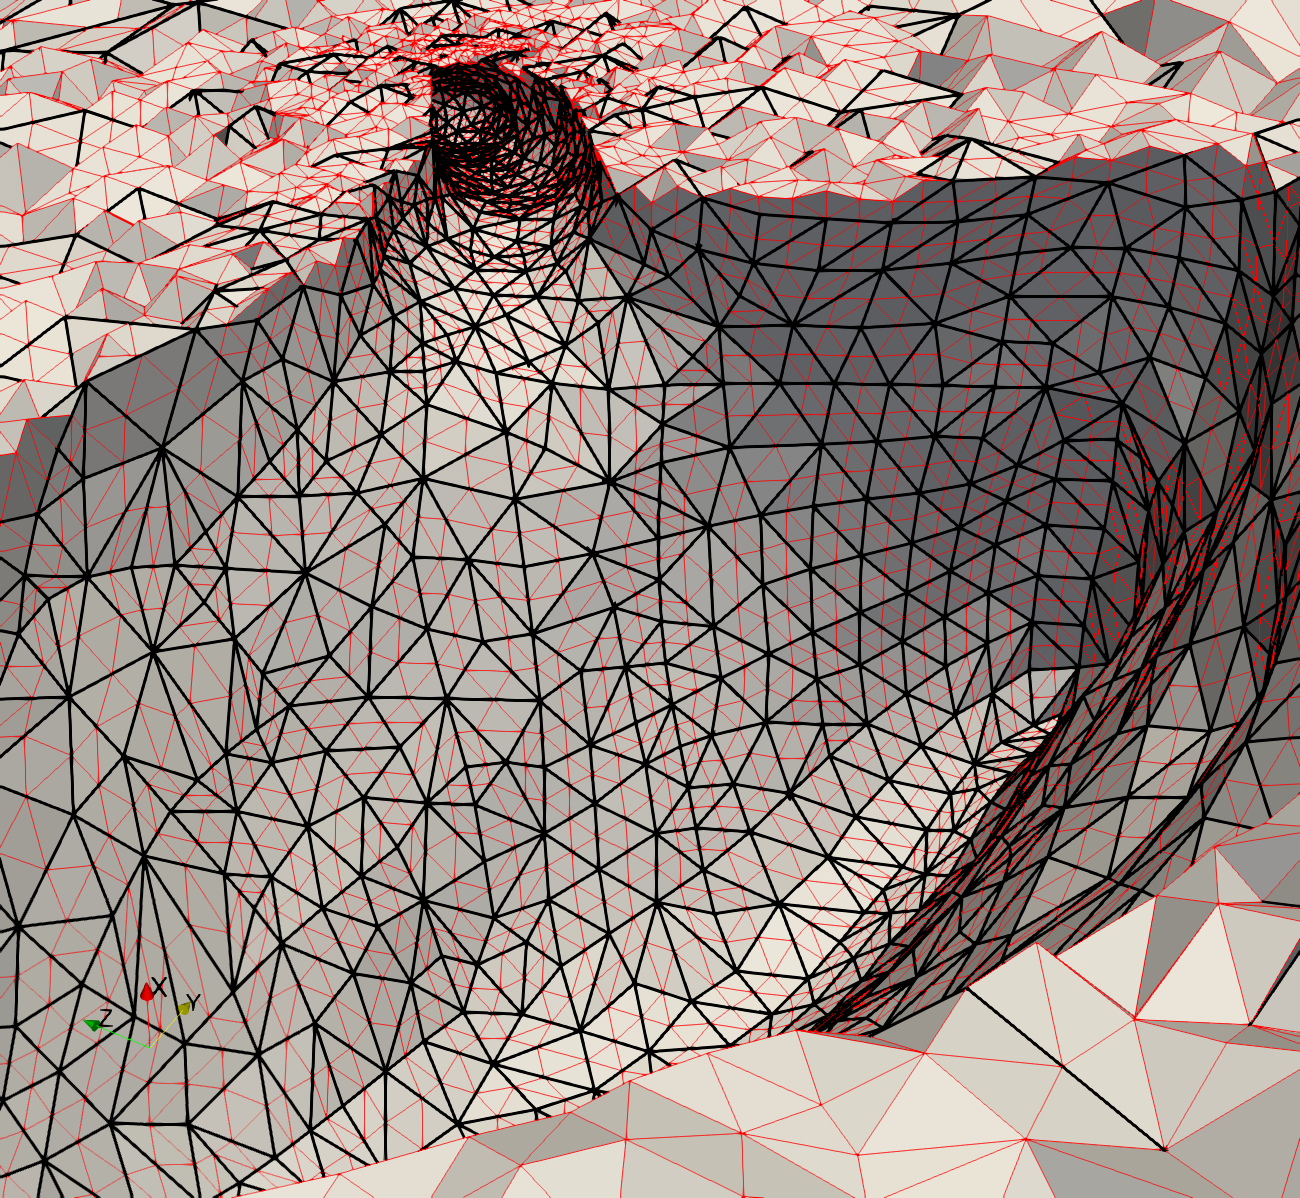
\includegraphics[width=0.5\textwidth]{img/aut_glial_nested}
\caption{Example of a nested mesh (red edges) obtained via a uniform
refinement of a base mesh (black edges) in three dimensions.}
\label{fig:aut_glial_nested}
\end{figure}

%%% DISCRETE ADJOINT APPROXIMATION
\subsection{Discrete Adjoint Approximation}

Let $\bs{R}^h : \mathbb{R}^n \to \mathbb{R}^n$ denote the residual form of
the system of nonlinear algebraic equations arising either from the Galerkin
\eqref{eq:aut_abstract_fem} or stabilized
\eqref{eq:aut_abstract_stabilized_fem}
model problem posed on the uniformly nested mesh. Let $\bs{u}^h_H :=
I^h_H \bs{u}^H$ denote the prolongation of the primal finite element solution
onto the richer space $\S^h$ via interpolation,
Let $J^h : \mathbb{R}^n \to
\mathbb{R}$ denote the discretization of the functional QoI on the
uniformly nested fine space. We approximate the adjoint problem
\eqref{eq:aut_abstract_adjoint} in a discrete manner
\cite{fidkowski2011review, venditti2000adjoint, venditti2002adjoint,
venditti2003adjoint}, by solving
%
%%
\begin{gather}
\left[ \frac{\partial \bs{R}^h}{\partial \bs{u}^h} \biggr|_{u^h_H}
\right]^T \bs{z}^h = \left[ \frac{\partial J^h}{\partial \bs{u}^h}
\biggr|_{u^h_H} \right]^T.
\label{eq:aut_discrete_adjoint}
\end{gather}
%
This allows us to automate the process of solving the adjoint problem, as
discussed below. Here $\bs{z}^h \in \mathbb{R}^n$ denotes the adjoint
solution vector on the nested discretization.

%%% AUTOMATED SOLUTION BASED ON RESIDUAL FORMULATION
\subsection{Automated Solution Based on Residual Formulation}

The construction of the Jacobian transpose matrix $\left[ \partial \bs{R}^h
/ \partial \bs{u}^h \right]^T$ is performed in the same automated manner as
the Jacobian for the primal problem. That is, for each element, we compute
consistent element tangent stiffness matrices via automatic differentiation
of element-level contributions to the residual vector. However, during the
\emph{scatter} phase of the template-based generic programming process,
we transpose the element-level tangent matrices and
sum them into global Jacobian adjoint matrix. The computation of the Jacobian
adjoint is done using the same templated code that is used to compute
the primal residual vector and the Jacobian matrix, as illustrated by
listings \ref{lst:presidual} and \ref{lst:stabresidual}.

Similarly, the construction of the functional derivative vector
$\left[ \partial J^h / \partial \bs{u}^h \right]^T$ is done by evaluating
derivatives of element-level contributions to the functional via automatic
differentiation. This results in element-level derivative vectors that are
then assembled into the global functional derivative vector. Listings
\ref{lst:aut_avg_u_qoi} and \ref{lst:aut_avg_vm_qoi} illustrate the
implementation of two quantities of interest in the Goal application. Once
the Jacobian transpose matrix and functional derivative vector have been
assembled, we solve the adjoint problem \eqref{eq:aut_discrete_adjoint} using
a sparse iterative solver in parallel.

%%% ERROR ESTIMATION
\section{Error Estimation}

%%% TWO LEVEL ERROR ESTIMATES
\subsection{Two-Level Error Estimates}

Following Venditti and Darmofal
\cite{venditti2000adjoint, venditti2002adjoint, venditti2003adjoint},
we review adjoint-based error estimation using two discretization levels.
The discrete residual form of the governing equations for a Galerkin
\eqref{eq:aut_abstract_fem} finite element method or a stabilized finite
element method \eqref{eq:aut_abstract_stabilized_fem} posed on the fine
space can be expressed as
%
%% aut_fine_resid
\begin{gather}
\bs{R}^h(\bs{u}^h) = \bs{0}.
\label{eq:aut_fine_resid}
\end{gather}
%

Taking Taylor expansions of the discrete residual $R^h$ evaluated on the
fine space and the discrete functional $J^h$ evaluated on the fine space
about the point $\bs{u}^h_H$ yields
%
%% aut_residual_taylor
\begin{gather}
\bs{R}^h(\bs{u}^h) = \bs{R}^h(\bs{u}^h_H) +
\left[ 
\frac{ \partial \bs{R}^h }{ \partial \bs{u}^h} \biggr|_{\bs{u}^h_H}
\right]
(\bs{u}^h - \bs{u}^h_H) + \dots
\label{eq:aut_residual_taylor}
\end{gather}
%
and
%
%
%% aut_functional_taylor
\begin{gather}
J^h(\bs{u}^h) = J^h(\bs{u}^h_H) +
\left[
\frac{ \partial J^h } { \partial \bs{u}^h} \biggr|_{\bs{u}^h_H}
\right]
(\bs{u}^h - \bs{u}^h_H) + \dots
\label{eq:aut_functional_taylor}
\end{gather}
%
respectively.

Using equation \eqref{eq:aut_fine_resid}, the discretization error
between the two spaces can be approximated to first order as
%
%% aut_disc_error_approx
\begin{gather}
(\bs{u}^h - \bs{u}^h_H) \approx
- \left[
\frac{ \partial \bs{R}^h } { \partial \bs{u}^h } \biggr|_{\bs{u}^h_H}
\right]^{-1}
\bs{R}^h (\bs{u}^h_H ),
\label{eq:aut_disc_error_approx}
\end{gather}
%
which can then be substituted into the functional Taylor expansion
\eqref{eq:aut_functional_taylor} to obtain the so-called
\emph{adjoint weighted residual}
%
%% 
\begin{gather}
J^h(\bs{u}^h) - J^h(\bs{u}^h_H) \approx  - \bs{z}^h \cdot \bs{R}^h(\bs{u}^h_H)
\label{eq:aut_adjoint_weighted_residual}
\end{gather}
%
where $\bs{z}^h$ is the solution to the adjoint problem
\eqref{eq:aut_discrete_adjoint}.

%%% MODIFIED FUNCTIONAL ERROR ESTIMATE
\subsection{Modified Functional Error Estimate}

Assume that the QoI converges at the rate $k$, such that
$J - J^h(\bs{u}^h_H) = c H^k$ and $J - J^h(\bs{u}^h) = ch^k$,
where $J$ denotes the exact value of the QoI. If the fine space
is obtained via uniform mesh refinement, then the ratio of the fine mesh size
to the coarse mesh size is given as $\frac{h}{H} = \frac12$. Consider the ratio
%
%% aut_ratio
\begin{gather}
\begin{aligned}
\frac{ J^h (\bs{u}^h) - J^h(\bs{u}^h_H) }{ J - J^h(\bs{u}^h_H) }
&= \frac{\left[ J - J^h(\bs{u}^h_H) \right] -
\left[ J - J^h(\bs{u}^h) \right] }
{ J - J^h(\bs{u}^h_H) } \\
&= \frac{c H^k - ch^k}{c H^k} \\
&= 1 - \left( \frac{h}{H} \right)^k \\
&= 1 - \left( \frac12 \right)^k
\end{aligned}
\end{gather}
%
in the limit as $H \to 0$ \cite{fidkowski2011review}. We call this
ratio $\alpha := 1 - (1/2)^k$. Let $\eta$ denote an approximation
to the functional error $J - J^h(\bs{u}^h_H)$. Let $\I$
denote the effectivity index given by
%
%% aut_effectivity
\begin{gather}
\I = \frac{\eta}{ J - J^h(\bs{u}^h_H) }.
\label{eq:aut_effectivity}
\end{gather}
%
We would like to obtain error estimates $\eta$ that lead to
effectivity indices of $\I = 1$ as $H \to 0$. To this end, we recall
$J^h(\bs{u}^h) - J^h(\bs{u}^h_H) \approx - \bs{z}^h \cdot
\bs{R}^h(\bs{u}^h_H)$ from equation \eqref{eq:aut_adjoint_weighted_residual}
to obtain the scaled adjoint weighted residual error estimate
%
%% aut_error_estimate
\begin{gather}
\eta = - \frac{1}{\alpha} \bs{z}^h \cdot \bs{R}^h(\bs{u}^h_H).
\label{eq:aut_error_estimate}
\end{gather}

%%% ERROR LOCALIZATION FOR GALERKIN METHODS
\subsection{Error Localization for Galerkin Methods}

Following the approach of Richter and Wick
\cite{richter2015variational}, we introduce a partition of unity $\phi_i$, such that
$\sum_i \phi_i = 1$, into the weighting function slot for the
error estimate to localize the error. In this work, the partition of unity is
realized as linear Lagrange basis functions. This yields
local error contributions $\eta_i$ at the $n_{vtx}$ mesh
vertices in the mesh.  Let $z^h \in \V^h$ be the finite element
solution obtained by solving the discrete adjoint problem
\eqref{eq:aut_discrete_adjoint}. We assume that this solution
well approximates the continuous adjoint problem \eqref{eq:aut_abstract_adjoint},
such that $z \approx z^h$. Let $z^H$ denote the interpolant of $z^h$
onto the coarse space $\V^H$. Recalling the error representation
\eqref{eq:aut_abstract_galerkin_error} for Galerkin finite elements,
we obtain partition of unity-based correction indicators $\eta_i$ in the following
manner
%
%% aut_galerkin_localization
\begin{gather}
J(u) - J(u^H) \approx
\sum_{i=1}^{n_{vtx}}
\underbrace{
- \R_g( (z^h - z^H) \phi_i \; ; \; u^H).
}_{\eta_i}
\label{eq:aut_galerkin_localization}
\end{gather}

%%% ERROR LOCALIZATION FOR STABILIZED METHODS
\subsection{Error Localization for Stabilized Methods}

Error localization for the stabilized finite element formulation
\eqref{eq:aut_abstract_stabilized_fem} proceeds in the same manner as the
previous section. Let $z^h \in \V^h$ denote the finite element solution
obtained by solving the discrete adjoint problem
\eqref{eq:aut_discrete_adjoint} and let $z^H$ denote the interpolant
of $z^h$ onto the coarse space $\V^H$. Introducing a partition of unity into the
error representation \eqref{eq:aut_abstract_stabilized_error} for stabilized
finite element methods with the approximation $z \approx z^h$ yields
the vertex-based correction indicators $\eta_i$:
%
%% aut_stabilized_localization
\begin{gather}
J(u) - J(u^H) \approx
\sum_{i=1}^{n_{vtx}}
\underbrace{
- \R_g( (z^h - z^H) \phi_i \; ; \; u^H) +
\R_{\tau}( z^H \phi_i \; ; \; u^H)
}_{\eta_i}
\label{eq:aut_stabilized_localization}
\end{gather}

Once correction indicators $\eta_i$ have been evaluated, an approximate
upper bound $\hat{\eta}$ for the error is computed by summing the absolute
value of the error contributions over all mesh vetrices
%
%% aut_upper_bound
\begin{gather}
\hat{\eta} = \sum_{i=1}^{n_{vtx}} | \eta_i |
\label{eq:aut_upper_bound}
\end{gather}

%%% AUTOMATED ERROR LOCALIZATION BASED ON RESIDUAL IMPLEMENTATION
\subsection{Automated Error Localization Based on Residual Implementation}

During the assembly of the adjoint problem
\eqref{eq:aut_discrete_adjoint}, the evaluation of element-level
contributions to the residual vector evaluated on the fine space
$\bs{R}^h(\bs{u}^h_H)$ are necessarily computed by the machinery
of forward automatic differentiation. Thus,
during the \texttt{scatter} phase for the adjoint problem computation,
we additionally sum element-level contributions to the fine residual
to assemble the global vector $\bs{R}^h(\bs{u}^h_H)$. This, along
with the solution $\bs{z}^h$ to the adjoint problem
\eqref{eq:aut_discrete_adjoint} provides enough
information to compute the adjoint-weighted residual estimate
\eqref{eq:aut_error_estimate} in an automated fashion.

Again, we let $z^h \in \V^h$ denote the finite element solution to
the discrete adjoint problem \eqref{eq:aut_discrete_adjoint} and let
$z^H$ denote the interpolant of $z^h$ onto the coarse space $\V^H$.
We refer again to Listings \ref{lst:presidual} and \ref{lst:stabresidual},
which illustrate implementations of Galerkin and stabilized semilinear
forms $\R_g$ and $\R_{\tau}$, respectively, in the Goal application.
Specifically, we remark that these residual evaluations contain
the evaluation of weighting functions and their derivatives, given with
calls to the methods \texttt{w->val(node)} and \texttt{w->grad(node, dim)},
respectively. To localize the error in an automated fashion, we override
the calls to these methods such that they return values of the adjoint
solution multiplied by a partition of unity. For instance, at a given
reference location $\bs{\xi}$ in a given element, the
partition of unity-based
weight for the Galerin residual $\R_g$ is computed as
%
\begin{gather}
\texttt{w->val(n)} = \left[ (z^h - z^H) \cdot \phi_n \right] \bigr|_{\bs{\xi}},
\end{gather}
%
and its corresponding gradient is computed as
%
\begin{gather}
\texttt{w->grad(n)} = \nabla \left[ ( z^h - z^H) \cdot \phi_n \right] \bigr|_{\bs{\xi}}.
\end{gather}
%
Similarly, for the stabilized residual $\R_{\tau}$, the
partition of unity-based adjoint
weight is computed as
%
\begin{gather}
\texttt{w->val(n)} = \left[ z^H \cdot \phi_n \right] \bigr|_{\bs{\xi}},
\end{gather}
%
and its corresponding gradient is computed as
%
\begin{gather}
\texttt{w->grad(n)} = \nabla \left[  z^H \cdot \phi_n \right] \bigr|_{\bs{\xi}}.
\end{gather}
%
In this manner, we have introduced partition of unity-based adjoint weights
that have the
same data type as the weights used for the computation of the primal and
adjoint problems.

Using the adjoint weights in the error localization evaluation results in
element-level residual vectors that correspond to contributions to the
localized correction indicators $\eta_i$.
During the \texttt{scatter} phase of the error localization evaluation, we
sum these element level contributions to the appropriate mesh vertices
to compute the localized correction indicators $\eta_i$.

%%% MESH ADAPTATION
\section{Mesh Adaptation}

Given localized correction indicators $\eta_i$ at mesh
vertices, we compute element-level correction indicators $\eta_e$ for
$e = 1,2,\dots, n_{el}$, where $n_{el}$ is the number of elements in the
coarse discretization, by interpolating the vertex-based indicators to
element centers and taking the result's absolute value.

We then specify a \emph{mesh size field} that defines the desired value
of edge lengths over the mesh. From a high-level, we would like to specify
this size field such that areas of the mesh that contribute strongly to
the error in the QoI are refined, and areas of the mesh that are
insensitive to the error are coarsened. Following Boussetta et al.
\cite{boussetta2006adaptive}, we specify a size field that attempts to
equidistribute the error in an output adapted mesh with $N$ target
elements. Let $p$ be the polynomial interpolant order for the chosen
finite element method. In the present setting, $p=1$. We first define
the global quantity $G$ as
%
%% aut_global_size_quantity
\begin{gather}
G = \sum_{e=1}^{n_{el}} ( \eta_e ) ^{\frac{2d}{2p+d}}.
\label{eq:aut_global_size_quantity}
\end{gather}
%
With this global quanity, new element sizes $H_e^{\text{new}}$ are
computed by scaling the previous element size $H_e$
%
%% aut_size_field
\begin{gather}
H_e^{\text{new}} = \left( \frac{G}{N} \right)^{\frac{1}{d}}
( \eta_e )^{\frac{-2}{2p + d}} H_e
\label{eq:aut_size_field}
\end{gather}
%
Finally, to prevent excessive refinement or coarsening in a single
adaptive step, we clamp the element size such that it is no
smaller than one quarter and no greater than twice the previous
element size. This clamping is performed to ensure that mesh adaptation
is being driven by accurate error indicators.
%
%% aut_size_clamping
\begin{gather}
\frac14 \leq \frac{H_e^{\text{new}}}{H_e} \leq 2.
\label{eq:aut_size_clamping}
\end{gather}

%%% QUANTITIES OF INTEREST
\section{Quantities of Interest}

In this section, we review three quantities of interest that we have
implemented in the Goal application. One benefit of the current automated
approach is that additional quantities of interest can be rapidly
prototyped and investigated with relative ease. Here, we refer to the
domain discretized by the finite element mesh as $\Omega$.

%%% POINT-WISE SOLUTION COMPONENT
\subsection{Point-Wise Solution Component}

First, we consider the evaluation of a component $u_i$ of the solution $u$
at a given spatial localtion $\bs{x}$. This functional can be expressed as
%
%% aut_pw_qoi
\begin{gather}
J(u) = \int_{\Omega} \delta ( \bs{x} - \bs{x}_0 ) \, u_i
\; \text{d} \Omega,
\label{eq:aut_pw_qoi}
\end{gather}
%
where $\delta$ is the Dirac delta function. We implement this quantity of
interest as a discrete delta function, such that the right-hand side for
the adjoint problem takes the form
%
%% aut_discrete_delta
\begin{gather}
\frac{\partial J^h}{\partial \bs{u}^h} =
\begin{bmatrix}
0 & 0 & \dots & 0 & 1 & 0 & \dots & 0 & 0
\end{bmatrix}.
\label{eq:aut_discrete_delta}
\end{gather}
%
For this implementation, a mesh vertex is always placed at the spatial
location $\bs{x}_0$, the QoI derivative vector is zeroed out, and we place a
one in the row of the QoI derivative vector that corresponds to the $i^{th}$
component of the solution at the vertex.

%%% AVERAGE SOLUTION OVER A SUBDOMAIN
\subsection{Average Solution Over a Sub-domain}

Next, we consider the average solution over a sub-domain
$\Omega_0 \subset \Omega$, which can be expressed as
%
%% aut_avg_u_qoi
\begin{gather}
J(u) = \int_{\Omega_0} \frac{1}{n_c} \sum_{i=1}^{n_c} u_i
\; \text{d} \Omega.
\label{eq:aut_avg_u_qoi}
\end{gather}
%
Here, $n_c$ denotes the number of components for the solution vector. As an
example, Listing \ref{lst:aut_avg_u_qoi} demonstrates the Goal implementation
for the QoI corresponding to the average displacement over a sub-domain.

\begin{lstlisting}[
float,
style=mystyle,
caption=Evaluation of the average displacement over a sub-domain,
label=lst:aut_avg_u_qoi]
template <typename ScalarT>
void AvgDisp<ScalarT>::at_point(
    apf::Vector3 const&, double w, double dv) {
  for (int i = 0; i < num_dims; ++i)
    this->elem_value += u->val(i) * w * dv;
  this->elem_value /= num_dims;
}
\end{lstlisting}

%%% AVERAGE VON-MISES STRESS OVER A SUBDOMAIN
\subsection{Average von-Mises Stress Over a Sub-domain}

Finally, specifically for mechanics problems, we consider the evaluation of
the von-Mises stress integrated over a sub-domain $\Omega_0 \subset \Omega$,
given as
%
%% aut_avg_vm_qoi
\begin{gather}
J(u) = \int_{\Omega_0} \sigma_{vm} \; \text{d} \Omega,
\label{eq:aut_avg_vm_qoi}
\end{gather}
%
where the von-Mises stress $\sigma_{vm}$ is defined as
%
%% aut_vm_defn
\begin{gather}
\sigma_{vm} := \sqrt{\frac32 \bs{\sigma}'_{ij} \bs{\sigma}'_{ij}}.
\label{eq:aut_vm_defn}
\end{gather}
%
Here summation over repeated indices is implied and
$\bs{\sigma}' = \bs{\sigma} - \frac13 \text{tr}(\bs{\sigma})\bs{I}$ denotes
the deviatoric part of the Cauchy stress tensor $\bs{\sigma}$. The von-Mises
stress is often used in yield criterion for elastoplastic constitutive models,
and is hence of particular interest for solid mechanics desing applications.

We note that this funciton $J(u)$ has sources of nonlinearities from the
deviatoric stress tensor $\bs{\sigma}'$ and further nonlinearites introduced
by the definition of the von-Mises stress, which includes the square of
deviatoric stress components and a square root operation. The linearization
and implementation of this QoI, as required for adjoint-based error
estimation, would be cumbersome at best without some kind of automated
approach. In contrast, Listing \ref{lst:aut_avg_vm_qoi}
illustrates the simplicity of the relevant
\texttt{C++} code that implements integration point contributions to this
specific QoI in the Goal application.

\begin{lstlisting}[
float,
style=mystyle,
caption=Evaluation of the average von-Mises stress over a sub-domain,
label=lst:aut_avg_vm_qoi]
template <typename ScalarT>
void AvgVM<ScalarT>::at_point(
    apf::Vector3 const&, double w, double dv) {
  auto sigma = model->get_cauchy();
  ScalarT vm = compute_von_mises<ScalarT>(sigma);
  this->elem_value += vm * w * dv;
}
\end{lstlisting}

%%% RESULTS
\section{Results}

%%% POISSONS EQUATION
\subsection{Poisson's Equation}

As a first example, we investigate error estimation and mesh adaptation
in Poisson's equation for the model problem
%
%% aut_poisson
\begin{gather}
\begin{cases}
\begin{aligned}
- \nabla^2 u &= f \quad && \bs{x} \in \Omega, \\
u &= 0 \quad && \bs{x} \in \partial \Omega.
\end{aligned}
\end{cases}
\end{gather}
%
This model problem leads to the Galerkin finite element method: find
$u^H \in \V^H$ such that $\R_g(w^H; u^H) = 0$ for all $w^H \in \V^H$.
Here the residual $\R_g$ is defined as
%
%% aut_poisson_fem
\begin{gather}
\R_g(w^H; u^H) := (\nabla w^H, \nabla u^H) - (w^H, f),
\end{gather}
%
and the space $\V^H$ is given by
%
\begin{gather}
\V^H := \{ u^h \in H^1(\Omega) :
u^H = 0 \; \text{on} \; \partial \Omega \, , \,
u^H |_{\Omega_e} \in \mathbb{P}^1 \}.
\label{eq:aut_poisson_space}
\end{gather}
%
Here $\Omega_e$ denotes an element in a decomposition of the
domain $\Omega$ into $n_{el}$ non-overlapping elements such that
$\cup_{e=1}^{n_{el}} \Omega_e = \Omega$ and
$\Omega_i \cap \Omega_j = \varnothing$ if $i \neq j$.
Additionally,  $\mathbb{P}^1$ denotes the space of piecewise linear
polynomials.

The domain is chosen to be
$\Omega := [-1,1] \times [-1,1] \setminus
[-\frac12, \frac12] \times [-\frac12, \frac12]$ as shown in
Figure \ref{fig:aut_poisson_meshes}. The data is chosen to be
$f=1$ and we consider a point-wise
QoI of the form
$J(u) = \int_{\Omega} \delta(\bs{x} - \bs{x}_0) u \, \text{d} \Omega$,
where the point of interest $\bs{x}_0$ is chosen to be
$\bs{x}_0 = (0.75, 0.75)$. This problem was initially studied in
the reference \cite{dealiistep14}, where the QoI was determined
to have a reference value of $J(u) = 0.0334474 \pm 1e\mbox{-}7$.
Presently, we demonstrate that our automated approach can
reproduce the results for traditional adjoint-based error estimation
found in \cite{dealiistep14}.

\begin{figure}[ht!]
\centering
\begin{subfigure}{.36\textwidth}
\centering
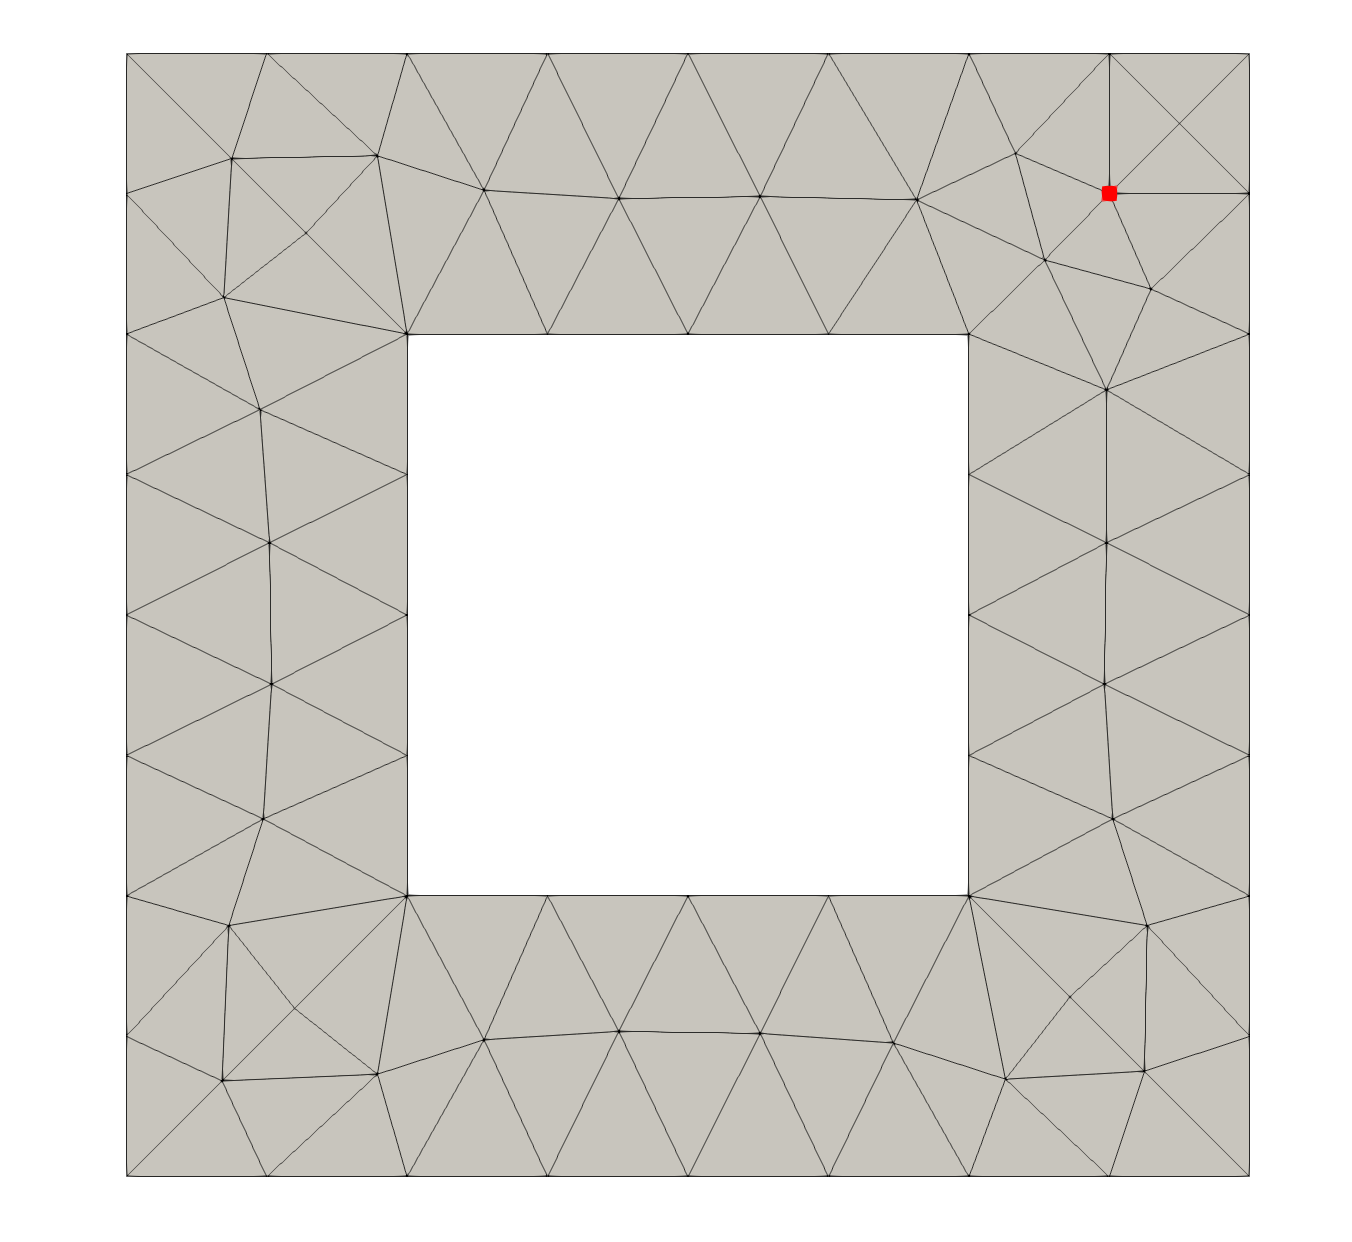
\includegraphics[width=.99\linewidth]{img/aut_squarehole_initial.png}
\end{subfigure}%
\begin{subfigure}{0.31\textwidth}
\centering
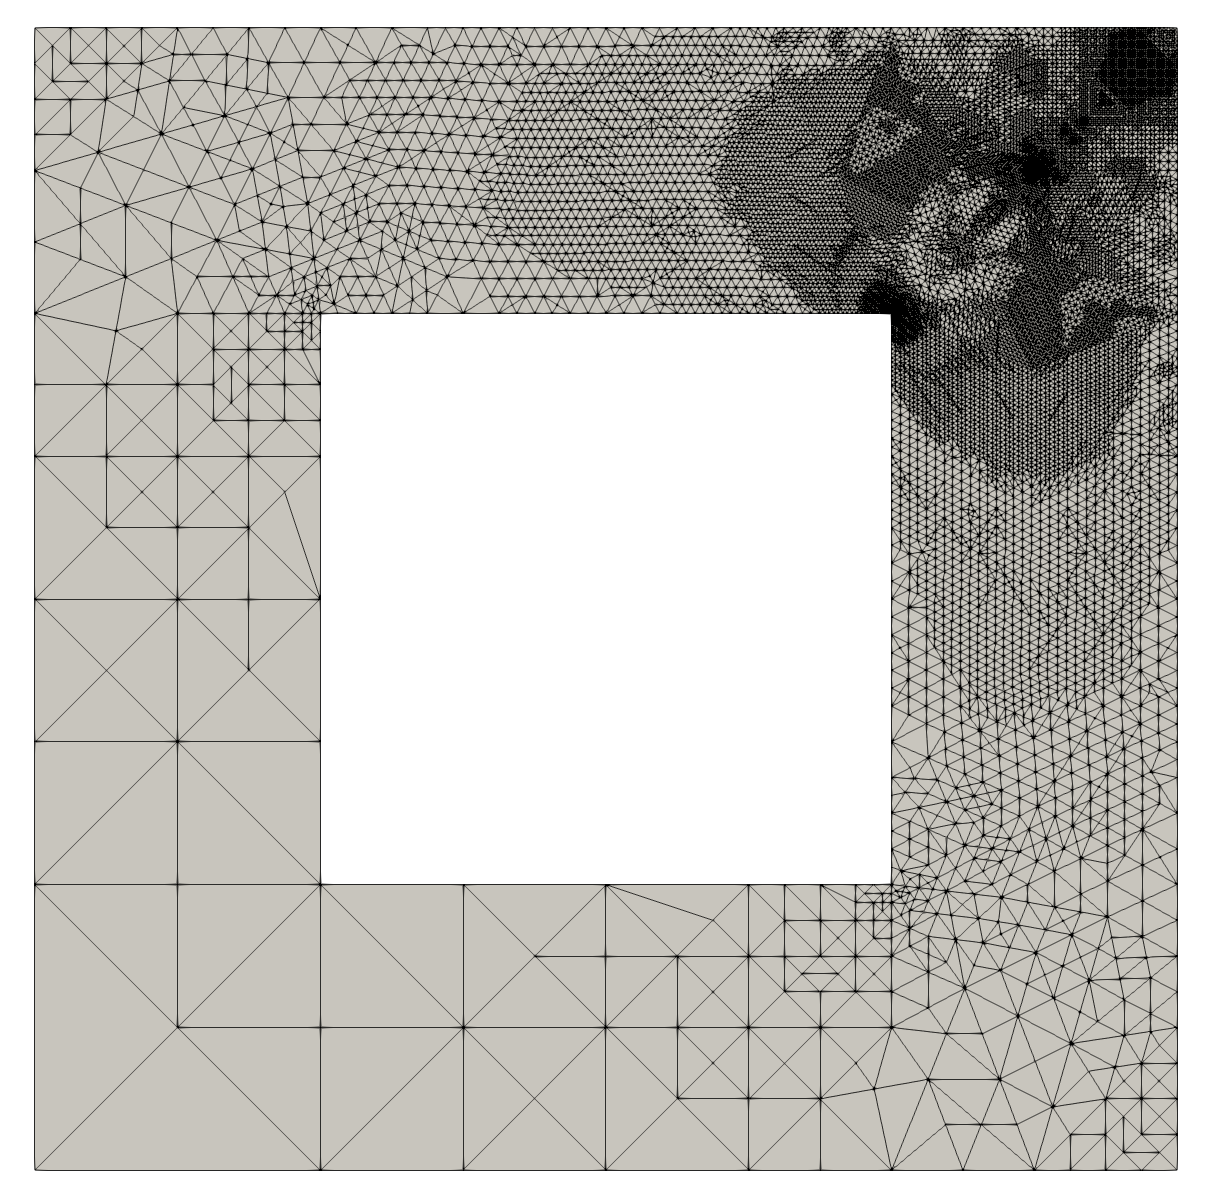
\includegraphics[width=.99\linewidth]{img/aut_squarehole_unif.png}
\end{subfigure}%
\begin{subfigure}{0.32\textwidth}
\centering
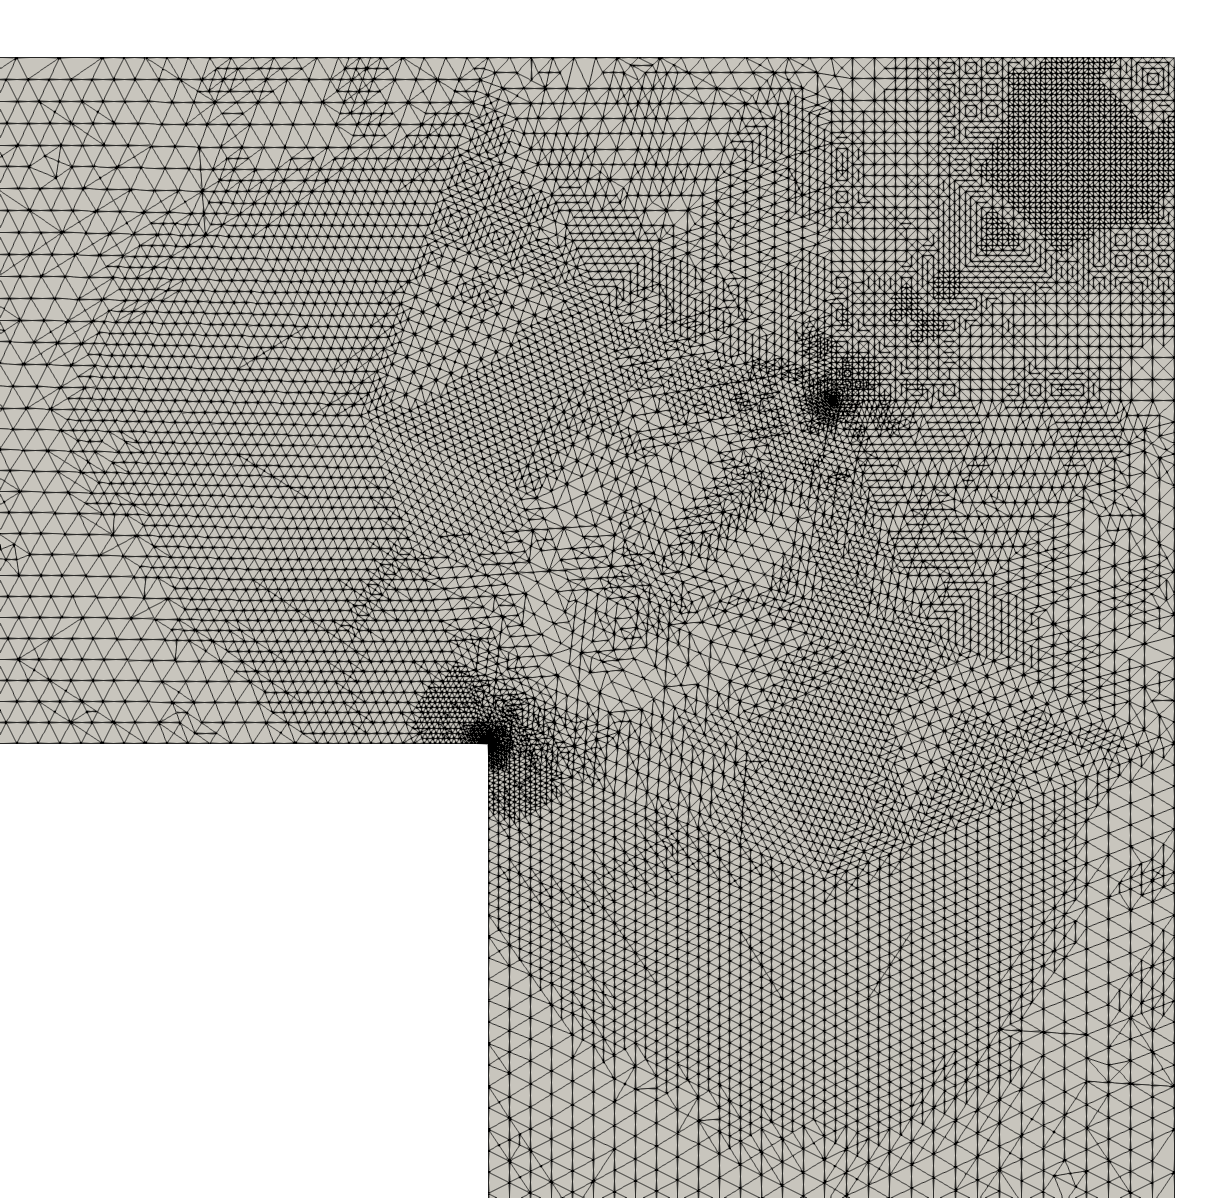
\includegraphics[width=.99\linewidth]{img/aut_squarehole_unif_close.png}
\end{subfigure}
\caption{Domain and initial mesh (left) for the Poisson's equation example
with the QoI point indicated in red, final adapted mesh (middle), and
a close up of the upper-right hand corner of the final adapted mesh (right).}
\label{fig:aut_poisson_meshes}
\end{figure}

Starting from the initial mesh shown in Figure \ref{fig:aut_poisson_meshes},
the steps:
%
\begin{gather*}
\text{Solve Primal} \rightarrow \text{Solve Adjoint} \rightarrow
\text{Estimate Error} \rightarrow \text{Adapt Mesh}
\end{gather*}
%
were performed seven times. The adaptive simulation was run using
4 MPI ranks. The mesh size field was set according to
equation \eqref{eq:aut_size_field} so that the target number of elements
is twice that of the current mesh. Figure \ref{fig:aut_poisson_meshes}
also shows the final adapted mesh resulting from this procedure. We remark
that the distribution of degrees of freedom in this mesh closely
resembles the results obtained in reference \cite{dealiistep14}.

%
%% aut_squarehole_effectivity
\begin{figure}[ht!]
\centering
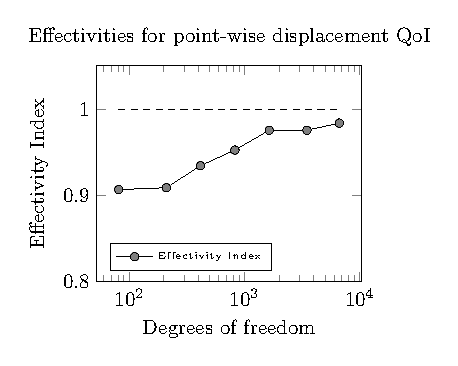
\includegraphics[width=.5\textwidth]{img/aut_squarehole_effectivity.pdf}
\caption{Effectivity indices for the adaptive Poisson's equation example.}
\label{fig:aut_squarehole_effectivity}
\end{figure}

We expect this functional to converge
at the rate $k=2$, such that the scaling factor $\alpha$ used in
the estimate \eqref{eq:aut_error_estimate} is given as
$\alpha = \frac34$. We consider the ``exact error''
$\E = J(u) - J(u^H)$ and the effectivity index
$\I = \frac{\eta}{\E}$, where $\eta$ is the estimate given by
equation \eqref{eq:aut_error_estimate}. Here we have placed quotations
around the term exact error because we have only approximated the
exact value of the QoI $J(u)$, and not truly recovered its exact value.
Figure \ref{fig:aut_squarehole_effectivity} plots the effectivity index
$\I$ versus the number of degrees of freedom in the adaptive
process. This plot demonstrates the ability of the error
estimate to recover the ``exact error'' as $H \to 0$.

%
%% aut_squarehole_error
\begin{figure}[ht!]
\centering
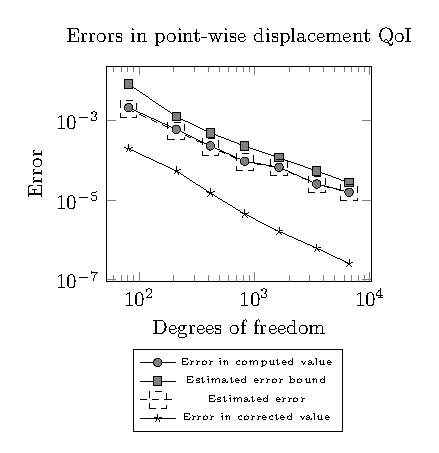
\includegraphics[width=.5\textwidth]{img/aut_squarehole_error.pdf}
\caption{Errors for the point-wise QoI for the adaptive Poisson's equation
example.}
\label{fig:aut_squarehole_error}
\end{figure}

Figure \ref{fig:aut_squarehole_error} displays the evolution of
various during the adaptive process. The ``exact error'' $\E$
and the estimated error $\eta$ are very close, as previously
demonstrated by the effectivity index $\I$. Additionally, the
approximated upper bound on the error $\hat{\eta}$ overestimates
the error, but not to a large degree. This provides some indication
that the correction indicators are effective in that they do
not drastically overestimate error. Finally, we remark that an
improved \emph{corrected} QoI functional value can be
computed as $J^*(u^H) = J(u^H) + \eta$. Figure
\ref{fig:aut_squarehole_error} demonstrates that this corrected
value is nearly an order of magnitude more accurate than
the computed functional value $J(u^H)$ during the adaptive process.

%
%% aut_squarehole_convergence
\begin{figure}[ht!]
\centering
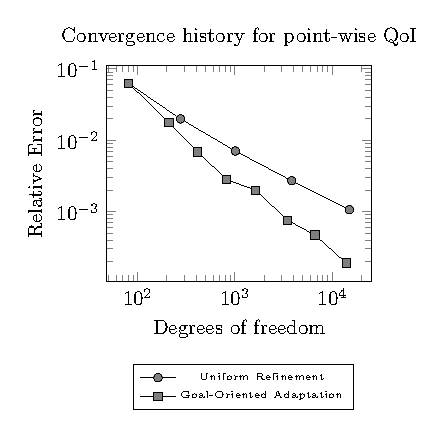
\includegraphics[width=.5\textwidth]{img/aut_squarehole_convergence.pdf}
\caption{Error convergence using uniform mesh refinement and adjoint-based
error estimation for the adaptive Poisson's equation example.}
\label{fig:aut_squarehole_convergence}
\end{figure}

Finally, Figure \ref{fig:aut_squarehole_convergence} demonstrates the
evolution of the ``exact error'' for two adaptive strategies.
The first strategy uniformly refines the mesh at each adaptive
step and the second strategy performs the adjoint-based adaptive scheme
developed in this work. We note that the error for the adjoint-based
adaptive scheme converges faster than the uniform refinement scheme.
Further, this convergence plot is consistent with the reference
\cite{dealiistep14}. 

%%% NONLINEAR ELASTICITY
\subsection{A Cell Embedded in a Matrix}

Recently, the automated approach developed in this paper was applied
to a stabilized mixed pressure-displacement finite element formulation
\cite{ramesh2005stabilized} for the governing equations of finite
deformation elasticity in a total Lagrangian setting
\cite{granzow2017adjoint} (see Chapter \ref{chap:mech}).
For two and three dimensional problems in
nonlinear elasticity, the automated approach was shown to effectively
estimate the error and provide improved error convergence rates via
adjoint-based mesh adaptation over uniform refinement.

In this section, the parallelization of a biomechanical application
presented in the reference \cite{granzow2017adjoint} is discussed. First,
the governing equations are briefly reviewed. For mixed pressure-displacement
formulations in the Goal application, the Galerkin residual is
defined as:
%
%% aut_mech_galerkin
\begin{gather}
\begin{aligned}
&\R_g(\bs{W}^H ; \bs{U}^H) := \\
&\int_{\Omega} \bs{P} : \nabla \bs{w}^H \, \text{d} \Omega +
\int_{\Omega} \left[ \frac{p^H}{\kappa} - \frac{1}{2 J}(J^2 - 1) \right] \;
q^H \, \text{d} \Omega -
\int_{\partial \Omega_h} \bs{h} \cdot \bs{w} \; \text{d} \Gamma,
\end{aligned}
\label{aut:mech_galerkin}
\end{gather}
%
and the stabilization residual is defined as:
%
%% aut_mech_stabilized
\begin{gather}
\R_{\tau}(\bs{W}^H ; \bs{U}^H) :=
\sum_{e=1}^{n_{el}} \int_{\Omega_e} \tau_e
(J \bs{F}^{-1} \bs{F}^{-T}) : (\nabla p^H \otimes \nabla q^H) \;
\text{d} \Omega.
\label{aut_mech_stabilized}
\end{gather}
%
Here, $\bs{F}$ is the deformation gradient, $J := \text{det}(\bs{F})$,
$\bs{h}$ is an applied traction over the boundary $\partial \Omega_h$,
$\bs{P} := J \bs{\sigma} \bs{F}^{-T}$ is the first Piola-Kirchhoff
stress tensor, $\bs{\sigma}$ is the Cauchy stress tensor, $n_{el}$
is the total number of elements in the mesh, and $\tau_e :=
\frac{c_0 H_e^2}{2 \mu}$ is a mesh-dependent stabilization parameter,
where $c_0$ is a non-negative stability constant, $H_e$ denotes an
element mesh size and $\mu$ denotes the bulk modulus.
The Cauchy stress tensor is defined via a neo-Hookean constitutive
relationship.  The total
solution vector is defined as $\bs{U}^H := [\bs{u}^H, p^H]$, where
$\bs{u}^H$ corresponds to displacements and $p^H$ corresponds to
pressures. Similarly, the total weighting vector is defined as
$\bs{W}^H := [\bs{w}^H, q^H]$, where $\bs{w}^H$ denotes a weighting
function corresponding to displacements and $q^H$ is a weighting
function corresponding to pressures. For a complete
exposition, we refer the reader to Chapter \ref{chap:mech}.

%
%% aut_glial_geom
\begin{figure}[ht!]
\centering
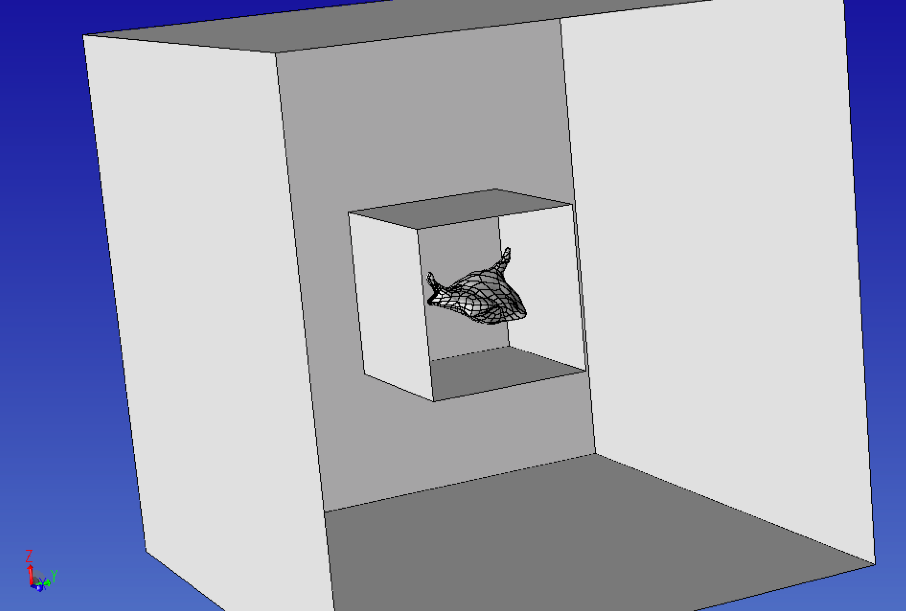
\includegraphics[width=.5\linewidth]{img/aut_glial_geom.png}
\caption{Domains for the microglial cell example.}
\label{fig:aut_glial_geom}
\end{figure}

We focus on a microglial cell with dimensions of about
$20 \mu m \times 20 \mu m \times 20 \mu m$ embedded in an extracellular
matrix of dimension $100 \mu \times 100 \mu m \times 100 \mu m$.
The QoI is chosen to be a local average displacement
$J(\bs{U}) = \int_{\Omega_0} \frac13 (u_x + u_y + u_z) \, \text{d} \Omega$,
defined over a box $\Omega_0$ with dimensions
$30 \mu m \times 30 \mu m \times 30 \mu m$
that bounds the microglial cell. Figure \ref{fig:aut_glial_geom} shows
the geometry defining the microglial cell, the bounding box
$\Omega_0$, and the extracellular matrix. The shear modulus
is defined as $\mu = 600$ Pa and Poisson's ratio is set to be
$\nu = 0.4999$.

To drive the problem, traction boundary conditions are imposed along
the surface of the microglial cell. The magnitude of the applied
traction $\bs{h}$ is defined to be 10 times the distance to the
center of the cell and its direction points inward towards the
cell center. This traction is consistent with observed physical
behavior \cite{dong2017recovery}. Displacements $u_x = 0$,
$u_y=0$, and $u_z=0$ are applied to the faces with constant
minimum $x$-coordinate value, constant minimum $y$-coordinate
value, and constant minimum $z$-coordinate value, respectively,
to constrain rigid body rotations and translations.

%
%% aut_glial_meshes
\begin{figure}[ht!]
\centering
\begin{subfigure}{.33\textwidth}
\centering
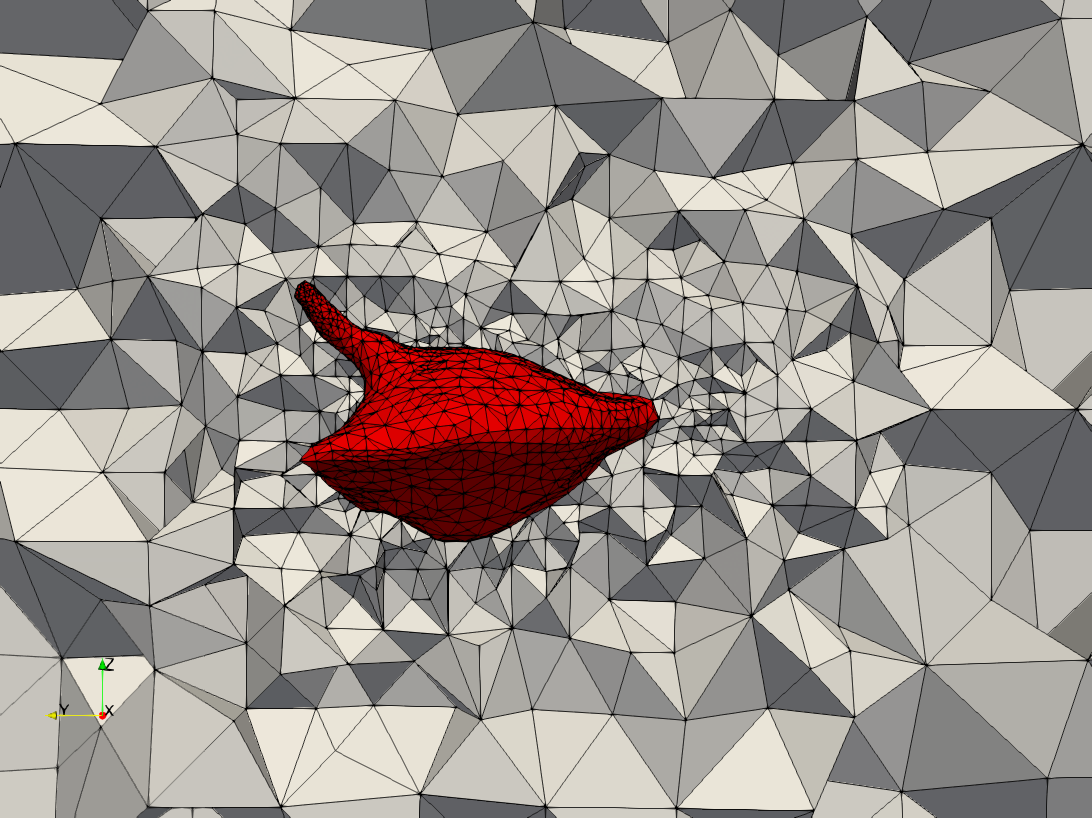
\includegraphics[width=.99\linewidth]{img/aut_glial_mesh0.png}
\end{subfigure}%
\begin{subfigure}{0.33\textwidth}
\centering
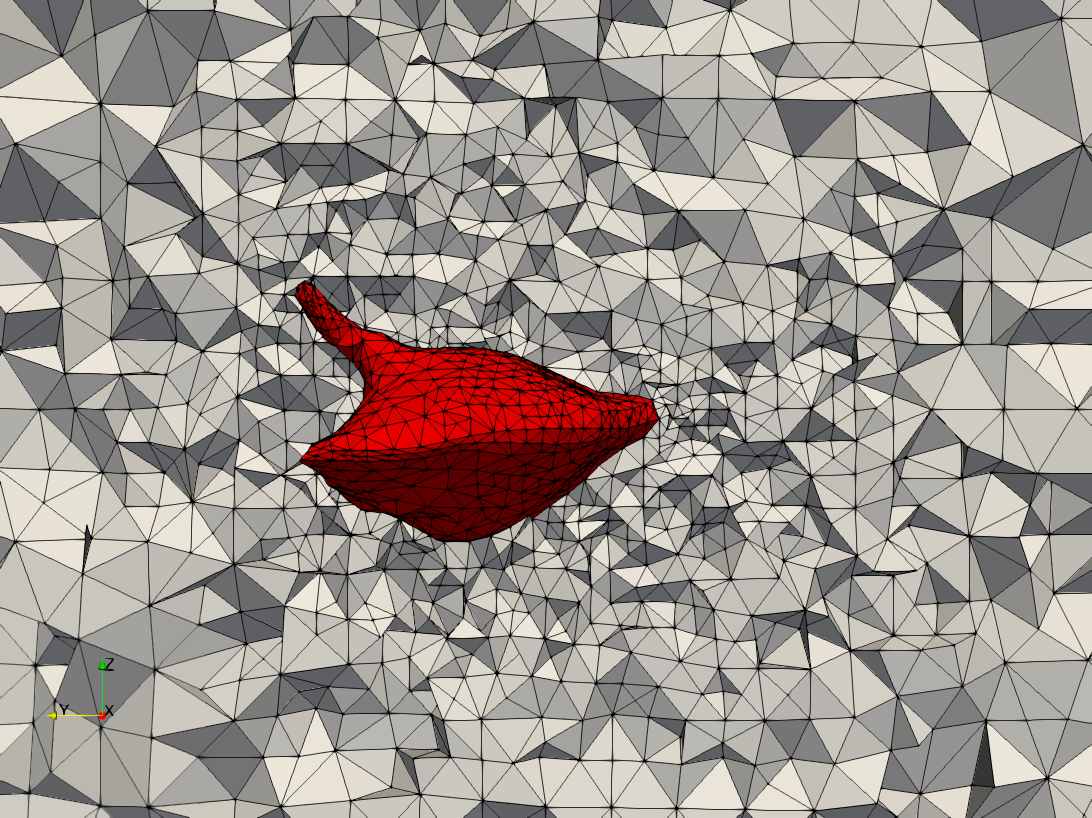
\includegraphics[width=.99\linewidth]{img/aut_glial_mesh5.png}
\end{subfigure}%
\begin{subfigure}{0.33\textwidth}
\centering
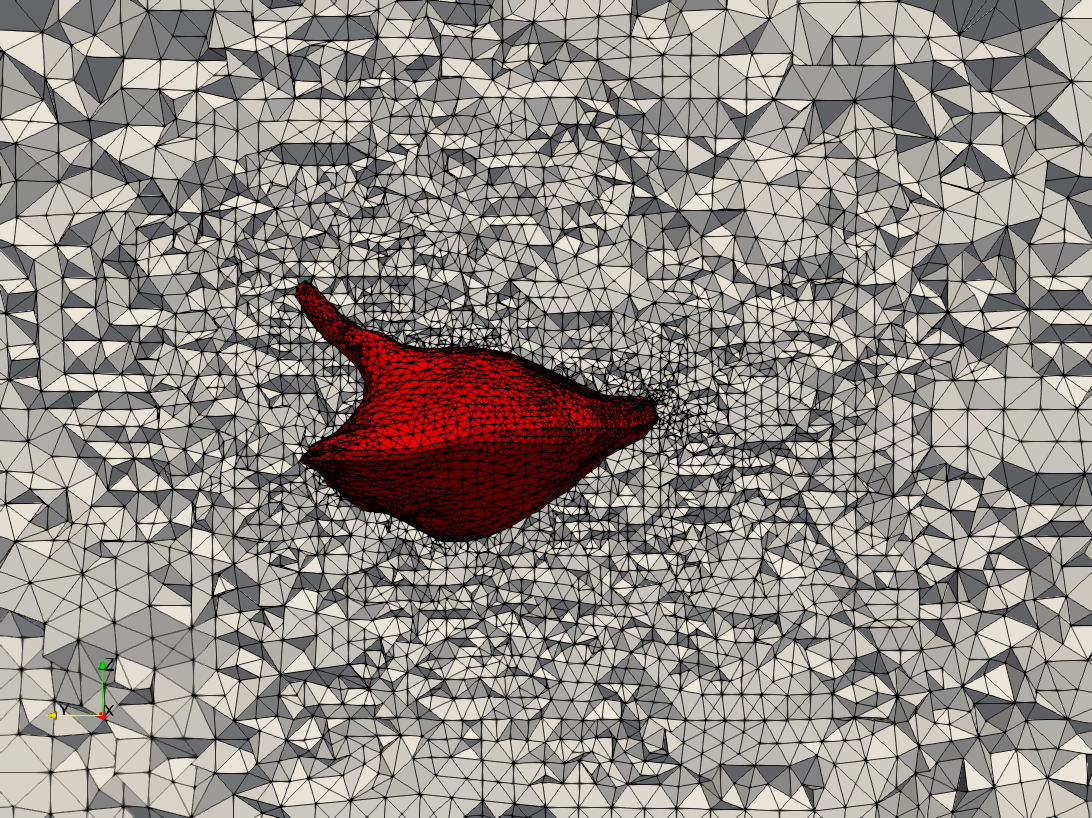
\includegraphics[width=.99\linewidth]{img/aut_glial_mesh10.png}
\end{subfigure}
\caption{A close-up of the initial mesh (left) the mesh after
5 adaptive iterations (center) and the final adapted mesh (right)
for the microglial cell example}
\label{fig:aut_glial_meshes}
\end{figure}

Figure \ref{fig:aut_glial_meshes} demonstrates an initial mesh,
which contains around $30,000$ degrees of freedom. From this initial
mesh, the steps
%
\begin{gather*}
\text{Solve primal PDE} \rightarrow
\text{Solve adjoint PDE} \rightarrow
\text{Localize error} \rightarrow
\text{Adapt mesh}
\end{gather*}
%
were successively performed $10$ times. During the adapt stage,
the mesh size field was set such that desired number of elements
$N$ in the output mesh is $1.5$ times the number of elements
in the previous mesh, according to equation \eqref{eq:aut_size_field}.
Figure \ref{fig:aut_glial_meshes} additionally demonstrates the adapted
meshes obtained at the fifth and final adaptive iteration.
In particular, both \emph{coarsening} and \emph{refinement} is performed
during the adaptive iterations.

\begin{figure}[ht!]
\centering
\begin{subfigure}{.5\textwidth}
\centering
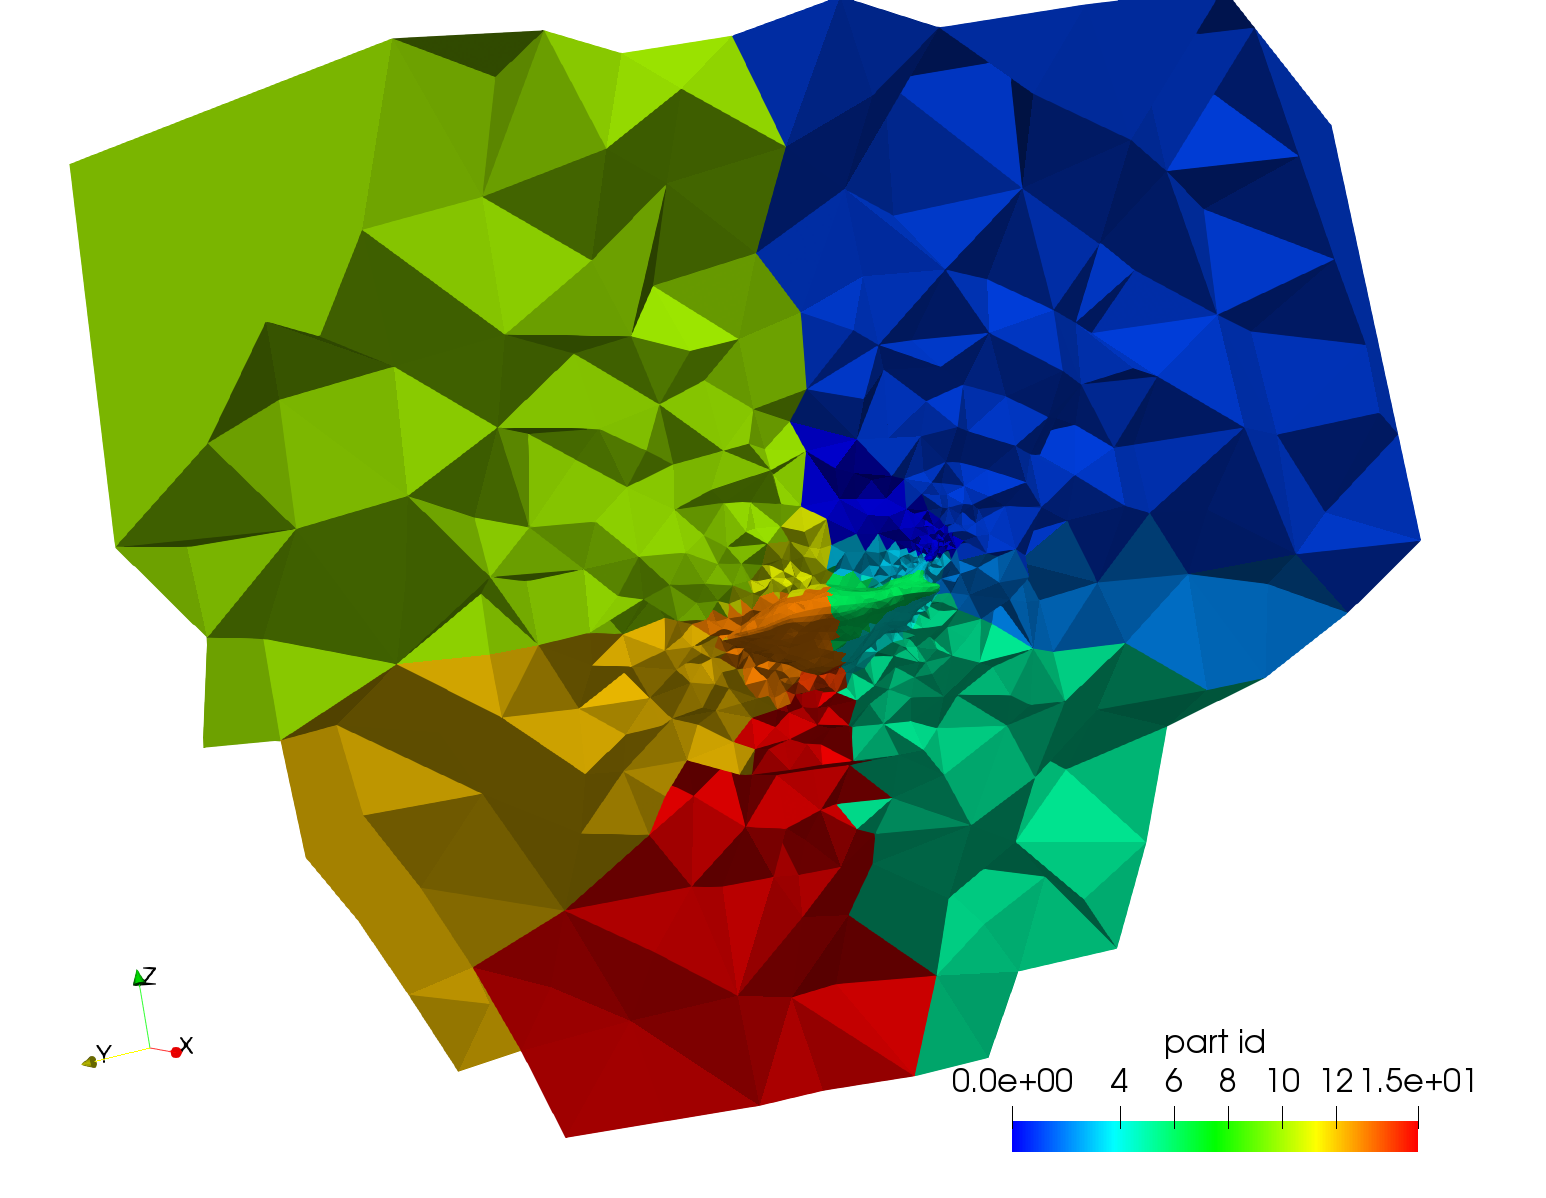
\includegraphics[width=.99\linewidth]{img/aut_glial_initial_parts.png}
\end{subfigure}%
\begin{subfigure}{0.5\textwidth}
\centering
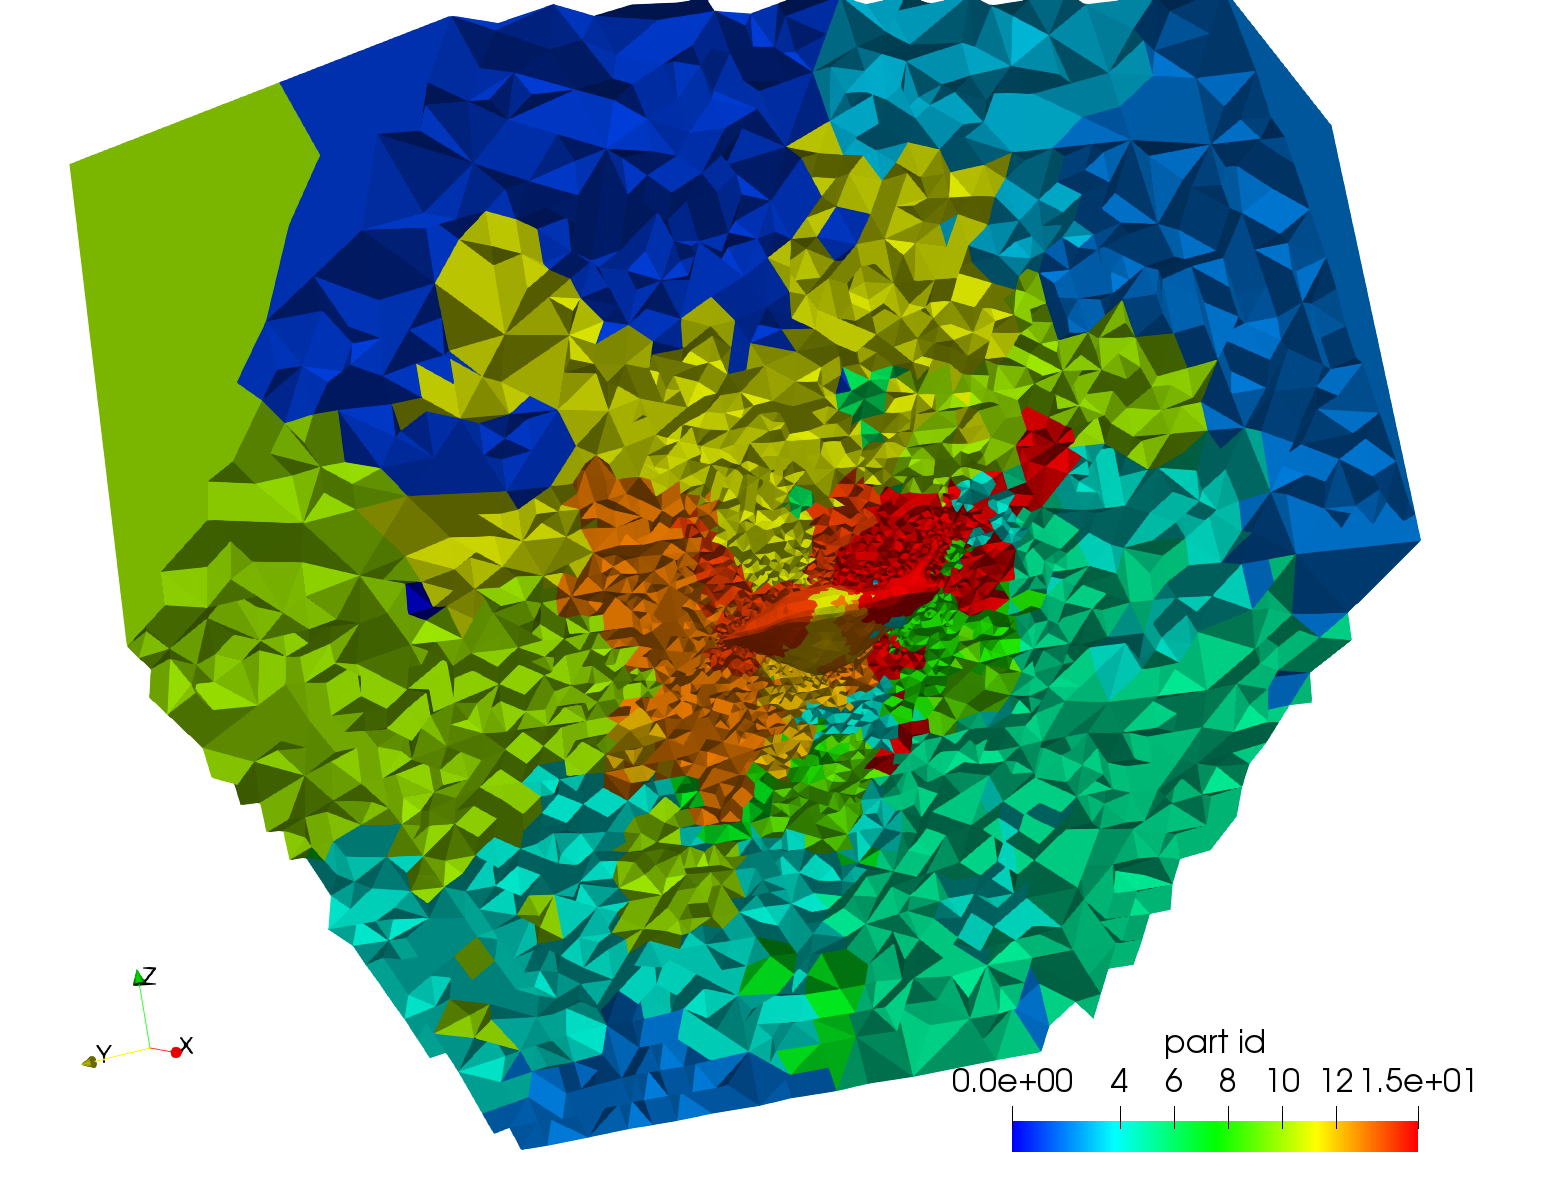
\includegraphics[width=.99\linewidth]{img/aut_glial_final_parts.png}
\end{subfigure}
\caption{The parallel mesh partitioning for the initial mesh (left)
and the final adapted mesh (right) for the microglial cell example}
\label{fig:aut_glial_parts}
\end{figure}

The problem was run using 16 MPI ranks. Figure \ref{fig:aut_glial_parts}
demonstrates the parallel partitioning for the initial mesh and for
the final adapted mesh obtained after 10 adjoint-based adaptive
iterations. To ensure partitioning quality, ParMA was
utilized to guarantee the imbalance of vertices and elements
across parallel partitions is no greater than $5\%$.

\begin{figure}[ht!]
\centering
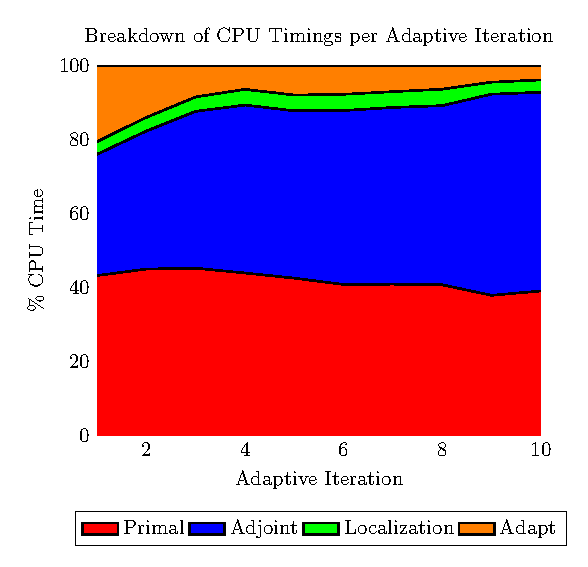
\includegraphics[width=0.4\linewidth]{img/aut_glial_timings.pdf}
\caption{Breakdown of the CPU time spent for each portion of
the adaptive process for the microglial cell example}
\label{fig:aut_glial_timings}
\end{figure}

Figure \ref{fig:aut_glial_timings} presents a breakdown of the
total percentange of CPU time spent on each step in the
adaptive analysis. For every adaptative iteration, the error
localization \eqref{eq:aut_stabilized_localization} takes only
a small percentage of the total CPU time, as it essentially amounts
to an evaluation of the residual vector the fine space. More
interestingly, mesh adaptation initially accounts for about
20 percent of the total CPU time but decreases as the adaptive
simulation progresses. This is explained by the fact that the initial
adaptive iteration requires more work to optimally distribute
the degrees of freedom for the functional QoI as compared to
subsequent adaptive iterations. In addition to refinement
and coarsening operations, the mesh adaptation step also
performs \emph{shape correction} to ensure elements are not
too heavily skewed \cite{li20053d}. Finally, we note that the
adjoint problem accounts for roughly 40 to 50 percent of the CPU time
over the course of the adaptive simulation. While process of
adjoint-based error estimation is not cheap for this example,
we provide two justifying remarks. First, this problem required only
3 to 4 Newton iterations for each primal solve. For constitutive
models with higher degrees of nonlinearity or for problems loaded to
higher strains, it is not uncommon for Newton's method to converge
in 7 to 10 iterations. In these scenarios, the relative cost of
adjoint-based error estimation is not as extreme.
Second, for this computational price, we have
achieved very accurate error estimates as shown in
Chapter \ref{chap:mech}.

%%% ELASTOPLASTICITY IN AN ARRAY OF SOLDER BALLS
\subsection{Elastoplasticity in an Array of Solder Joints}

In this section, we investigate the utility of adjoint-based mesh
adaptation for a thermomechanical analysis of an array of solder
joints used in microelectronics fabrication. We consider a
$6 \times 6$ array of solder joints sandwiched between two materials
with distinct thermomechanical properties
to model a portion of the process of `flip-chip'
manufacturing \cite{bloomfield2017component}. The full geometry
is shown in Figure \ref{fig:aut_solder_geom}. We consider
an elastoplastic constitutive model with a von-Mises yield
surface and linear isotropic hardening, as given by
Simo and Hughes \cite{simo1998computational} with a temperature
correction for the stress tensor \cite{li2017simulation}. The top
slab, solder joints, and bottom slab are modeled with the
distinct material properties given in reference
\cite{bloomfield2017component}.

To drive the problem, the entirety of the domain is cooled
from a reference temperature $T_{ref} = 393K$ to a
resting temperature of $T_{f} = 318K$ in a single load
step. The faces with minimum $x$, $y$, and $z$ coordinate
values were constrained to have zero displacements in
the $x$, $y$, and $z$ directions, respectively. As a
QoI, we consider the average von-Mises stress given by
equation \eqref{eq:aut_avg_vm_qoi} over three solder joints
shown in yellow in Figure \ref{fig:aut_solder_geom}.

\begin{figure}[ht!]
\centering
\begin{subfigure}{.5\textwidth}
\centering
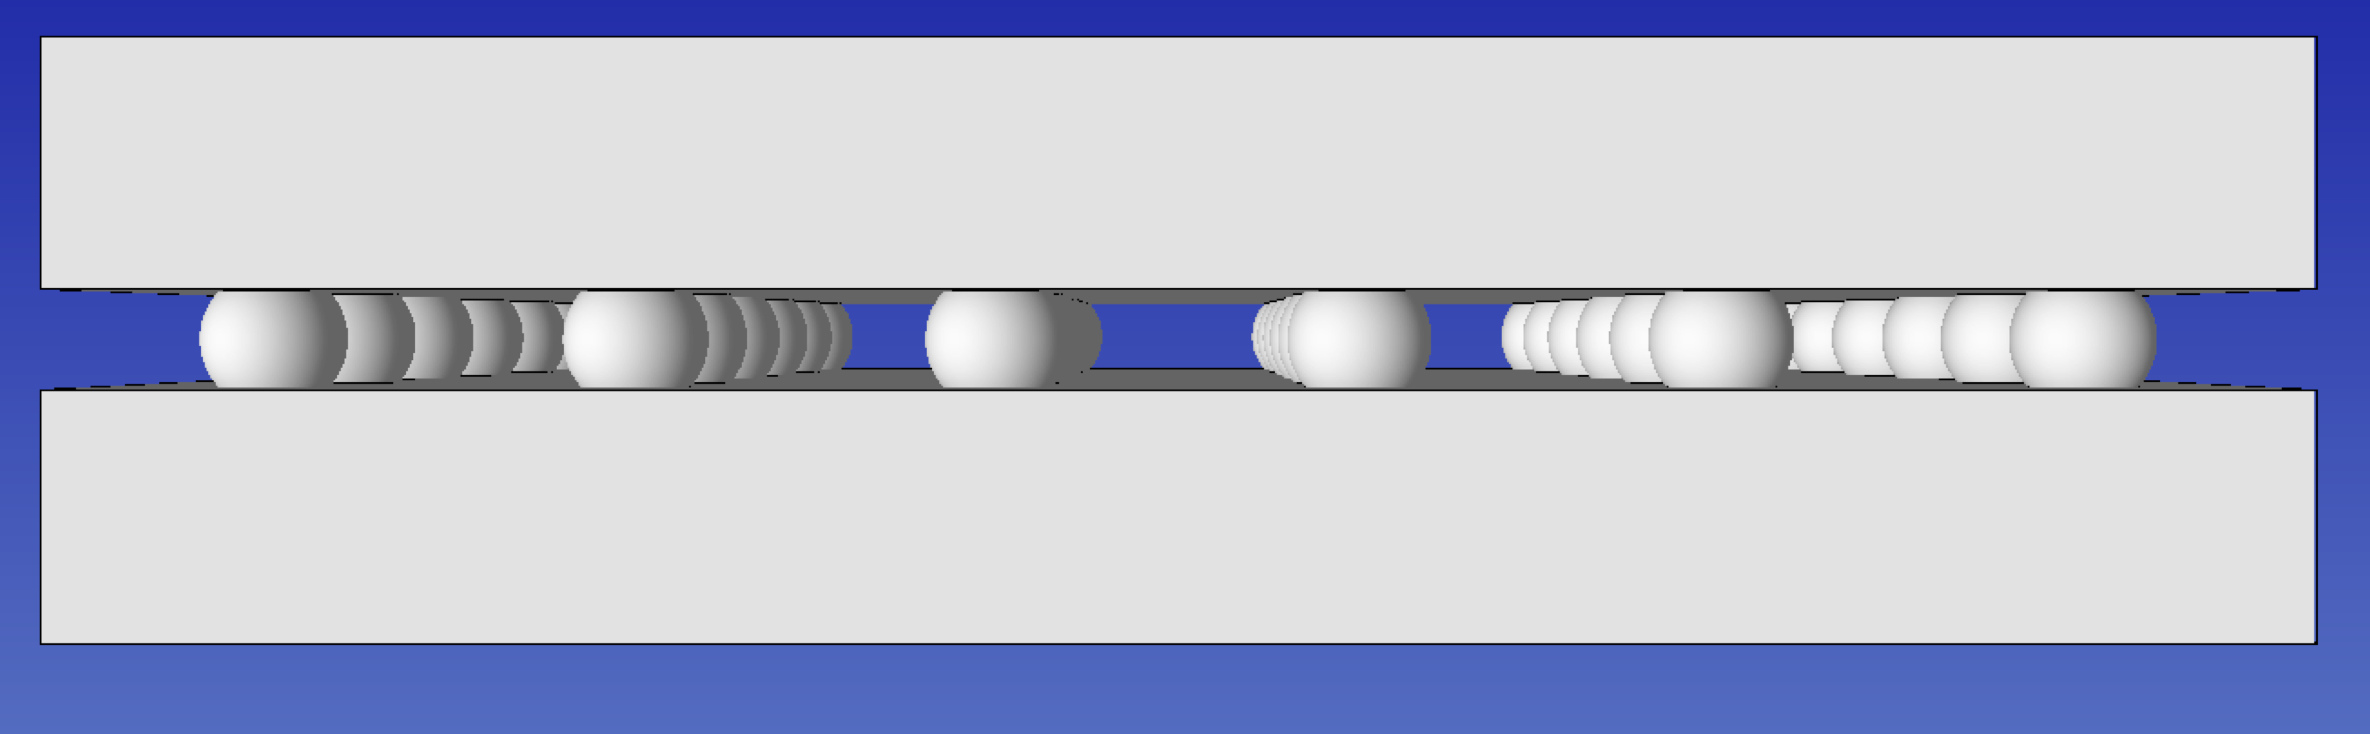
\includegraphics[width=.99\linewidth]{img/aut_solder_geom.png}
\end{subfigure}%
\begin{subfigure}{0.5\textwidth}
\centering
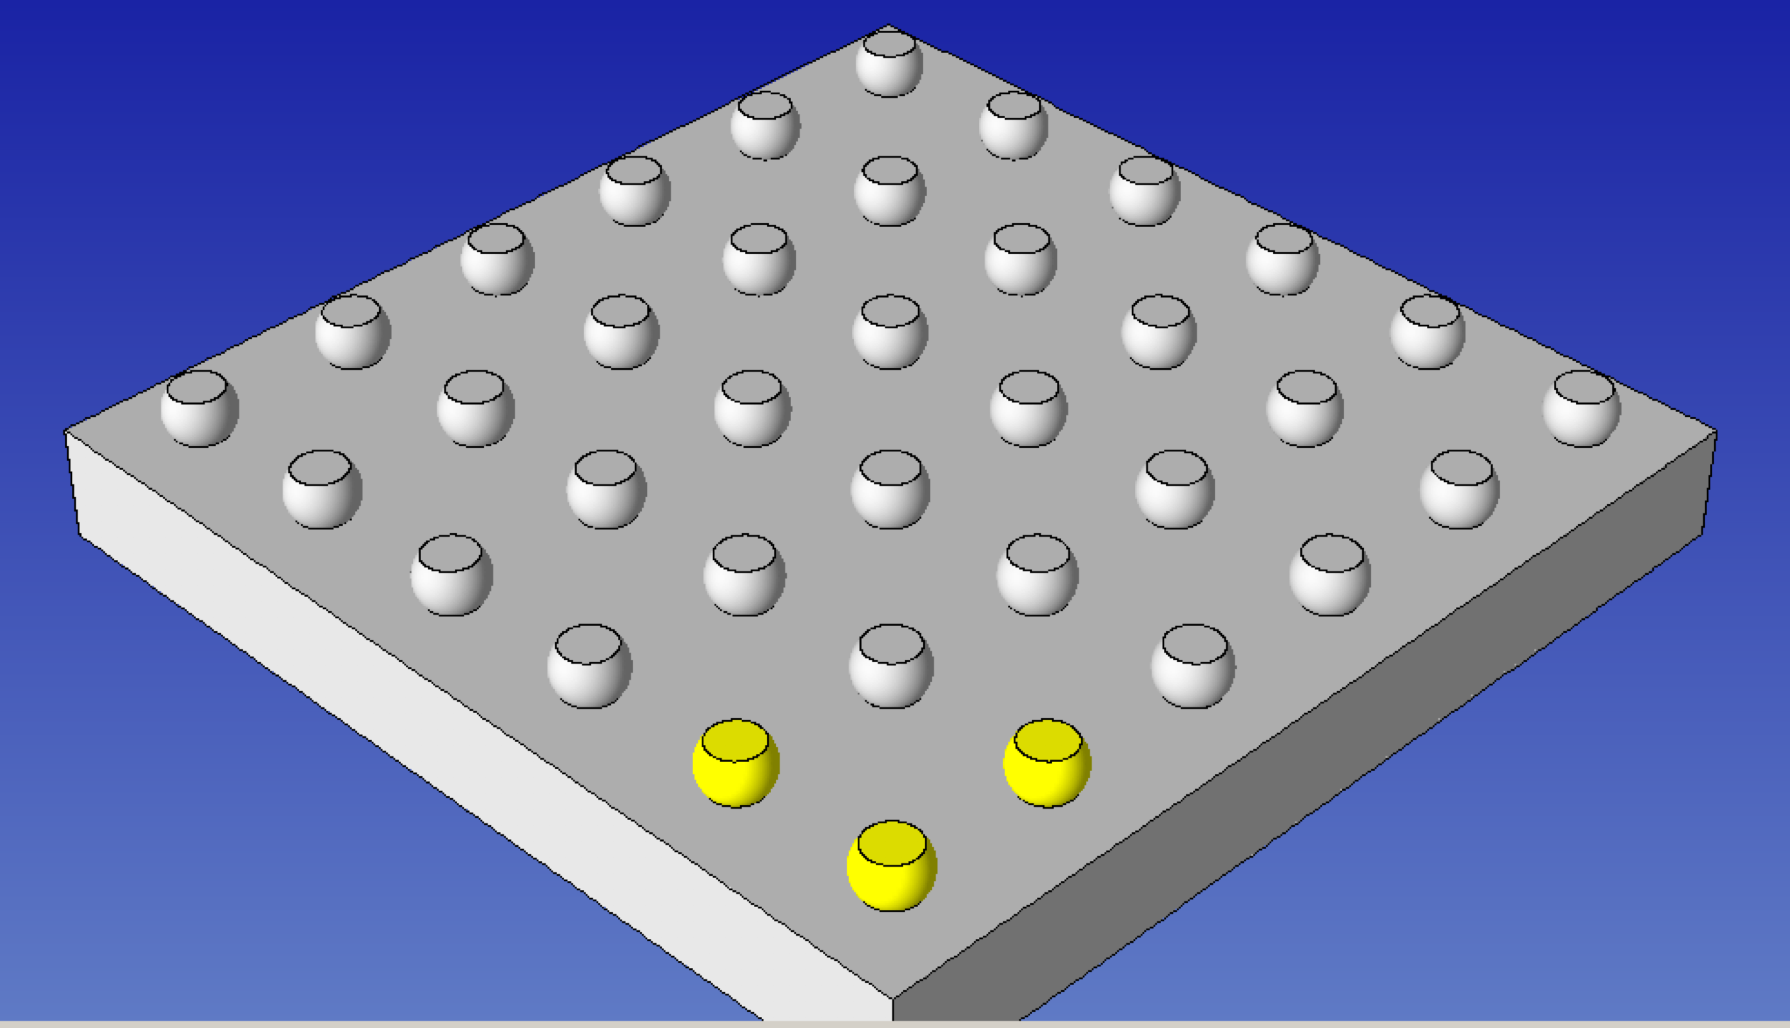
\includegraphics[width=.99\linewidth]{img/aut_solder_qoi_geom.png}
\end{subfigure}
\caption{The solder joint array geometry (left) and the
geometric specification of the average von-Mises QoI
(right).}
\label{fig:aut_solder_geom}
\end{figure}

The primal problem was solved on a sequence of uniformly refined
meshes, starting with an initial mesh with about 1 million
elements distributed over 16 MPI ranks, and finalizing with a
mesh with over half a billion elements distributed over
8192 MPI ranks. For each solve, the work load for each mesh
part (MPI rank) was held constant at approximately
$70,000$ elements. Figure \ref{fig:aut_weak_scaling}
demonstrates weak scaling timing results for various aspects
of the primal solve. In particular, we remark that the
assembly of the residual vector and Jacobian matrix scale
well as the number of MPI ranks increases. The preconditioning
routine shows a slight increase in time as the number of
MPI ranks increases, but this increase is not drastic.
The time to solve the linear system, however, does not scale
optimally. Improvements to parallel performance could likely
be made by more finely tuning the preconditioning and linear
solver routines for the specific problem, but this is outside
the scope of the present work.

\begin{figure}[ht!]
\centering
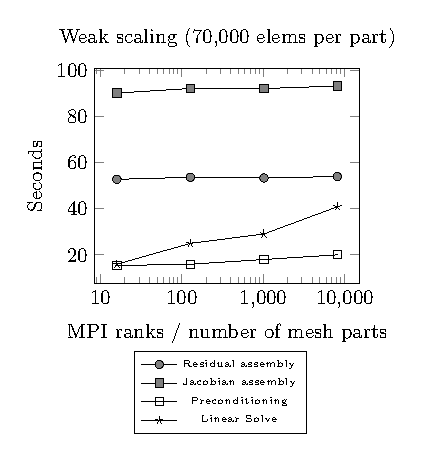
\includegraphics[width=0.5\linewidth]{img/aut_weak_scaling.pdf}
\caption{Weak scaling for the Goal application.}
\label{fig:aut_weak_scaling}
\end{figure}

The approximate QoI, $J^H(\bs{u}^H)$, was computed at each
primal solve. Using the QoI evaluations from the finest three meshes,
we performed Richardson extrapolation \cite{richardson1911approximate}
to obtain a more accurate representation of the QoI.
This value was given as $J(u) = 328.9$. We consider the extrapolated
value to be the ``true'' QoI value and measure errors with respect
to it. The expected convergence rate of the QoI is $k=1$, which is
confirmed by the Richardson extrapolation procedure.

\begin{figure}[ht!]
\centering
\begin{subfigure}{.33\textwidth}
\centering
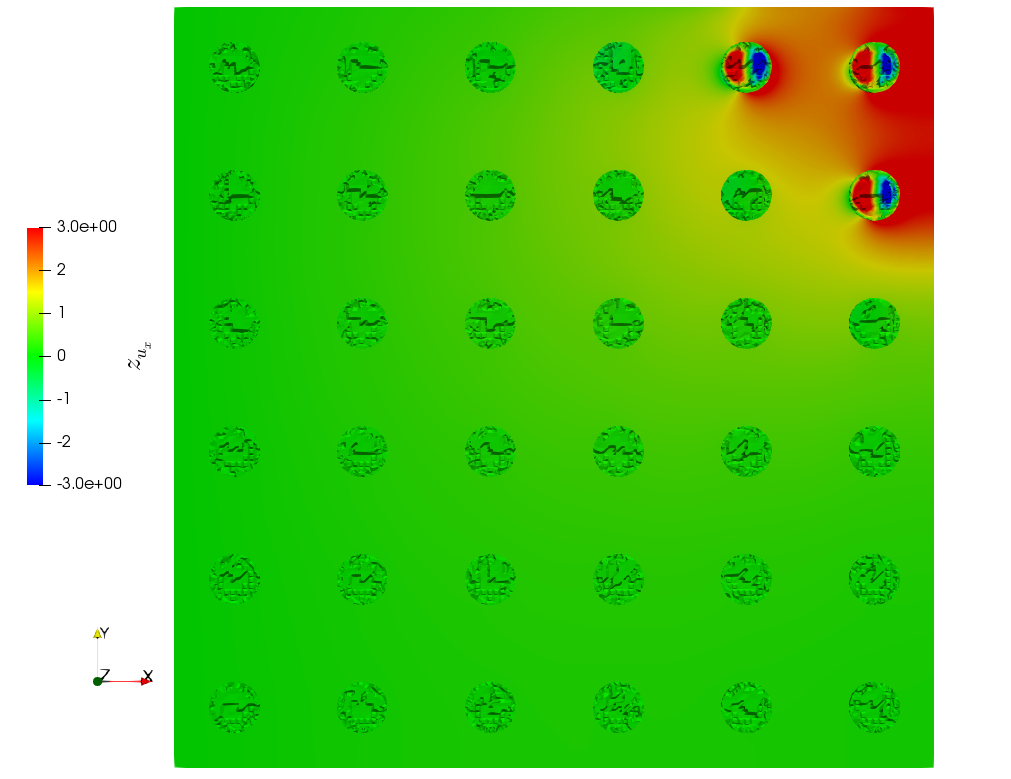
\includegraphics[width=.99\linewidth]{img/aut_solder_zux.png}
\end{subfigure}%
\begin{subfigure}{0.33\textwidth}
\centering
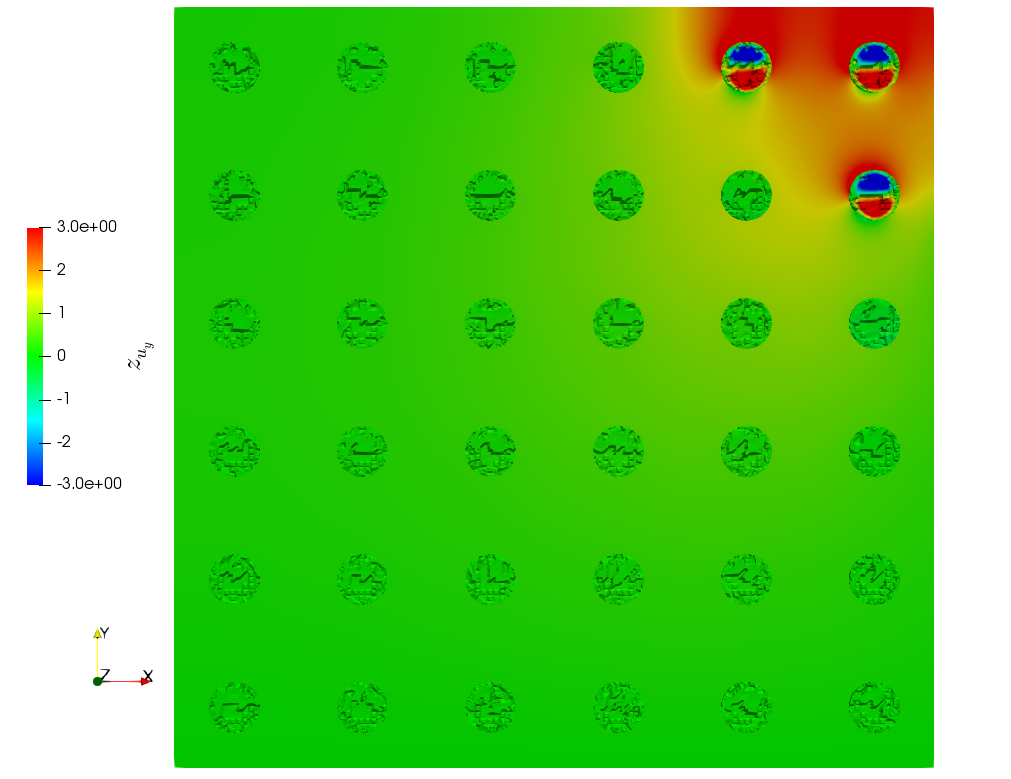
\includegraphics[width=.99\linewidth]{img/aut_solder_zuy.png}
\end{subfigure}%
\begin{subfigure}{0.33\textwidth}
\centering
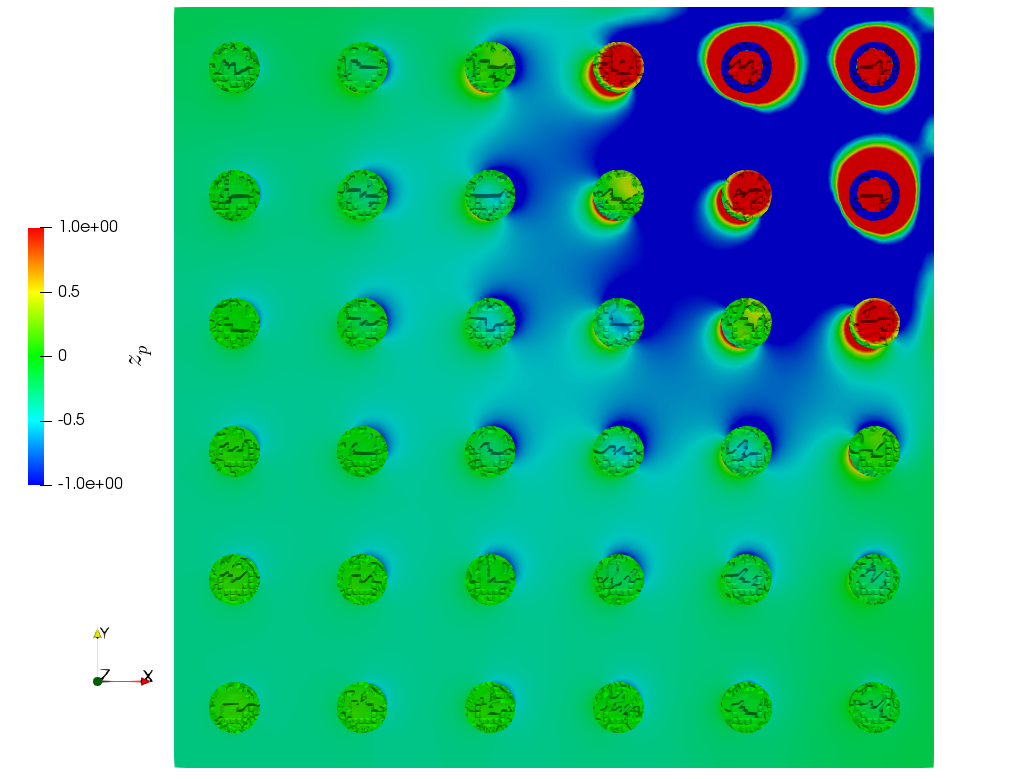
\includegraphics[width=.99\linewidth]{img/aut_solder_zp.png}
\end{subfigure}
\caption{The $x$-component of the adjoint displacement solution
(left), the $y$-component of the adjoint displacement solution
(center), and the pressure component of the adjoint solution
(right).}
\label{fig:aut_solder_adjoint}
\end{figure}

From the same initial mesh used in the weak scaling study,
we iteratively performed the steps:
%
\begin{gather*}
\text{Solve Primal} \rightarrow \text{Solve Adjoint} \rightarrow
\text{Estimate Error} \rightarrow \text{Adapt Mesh}
\end{gather*}
%
with a restart after each mesh adaptation using $128$,
$256$, and $512$ MPI ranks, such that the output number
of elements $N$ in the adapted mesh was targeted to be
$1$ million, $2$ million, and $4$ million elements,
respectively. Figure \ref{fig:aut_solder_adjoint} shows
different components of the adjoint solution obtained
during the adjoint-based adaptive process.
Figure \ref{fig:aut_solder_error} shows
the spatial distribution of the error for the given
QoI as computed by the adjoint-based error estimation process.
Unsurprisingly, the majority of the error is localized to the
area which geometrically defines the QoI. However, there are
also contributions to the error from nearby solder joints that
decrease as the distance from the 3 QoI solder joints
increases. These additional contributions to the error
are mostly gathered at the interface between solder
joints and the underlying material slab, where von-Mises
stress concentrations exist.

\begin{figure}[ht!]
\centering
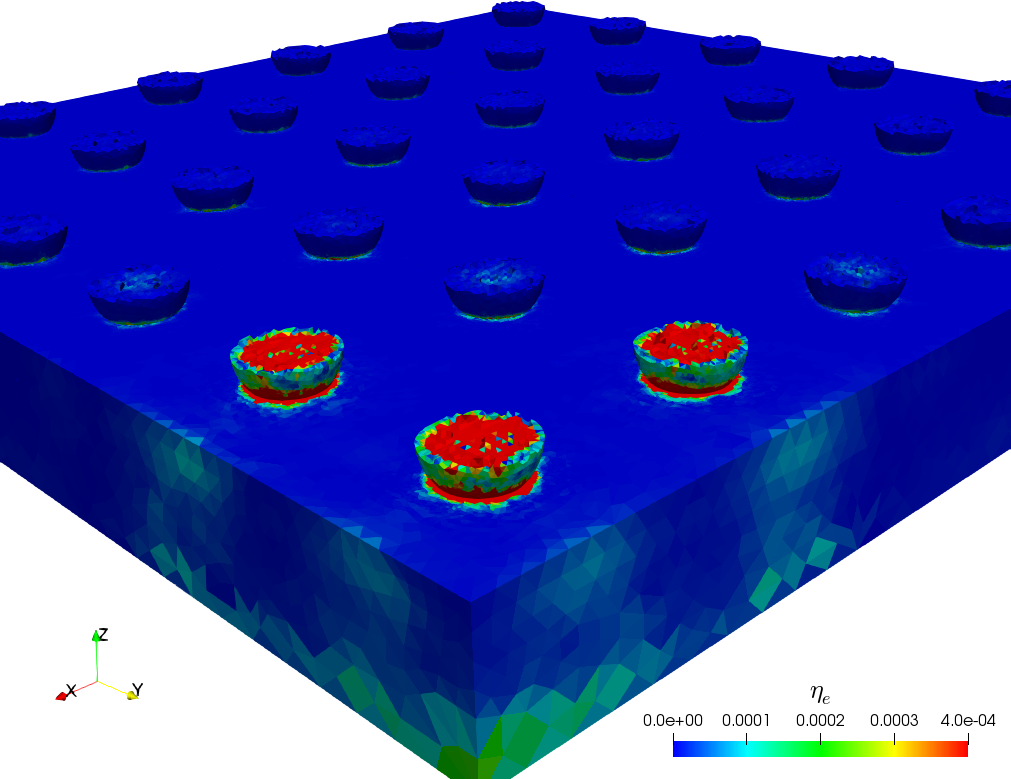
\includegraphics[width=.5\linewidth]{img/aut_solder_error.png}
\caption{The spatial distribution of errors as computed by
adjoint-based error estimation for the solder joint array.}
\label{fig:aut_solder_error}
\end{figure}

Figures \ref{fig:aut_solder_mesh} and \ref{fig:aut_solder_mesh2}
demonstrate the intial mesh used for the solder joint problem
and the final adapted mesh obtained via adjoint-based adaptation.
These figures clearly demonstrate that the 3 solder joints
that define the QoI sub-domain are heavily refined, as expected.
Additionally, notice that Figure \ref{fig:aut_solder_mesh}
demonstrates that there is refinement at the left-most solder joint,
which is not included in the geometric definition of the QoI.
The adjoint-based error estimation procedure indicates that
mesh must be refined in additional areas to accurately assess
the QoI.

\begin{figure}[ht!]
\centering
\begin{subfigure}{.5\textwidth}
\centering
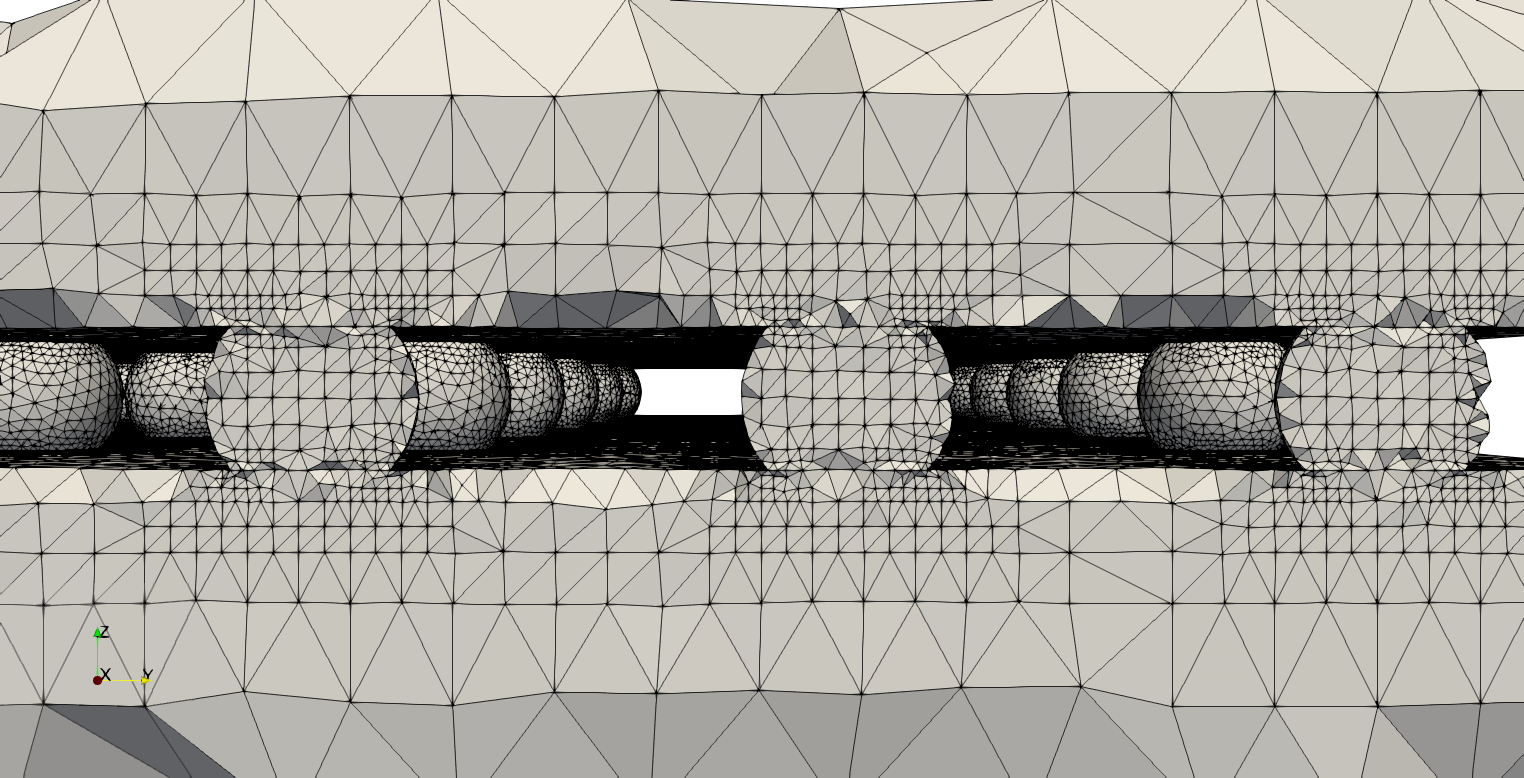
\includegraphics[width=.99\linewidth]{img/aut_solder_mesh_initial.png}
\end{subfigure}%
\begin{subfigure}{0.5\textwidth}
\centering
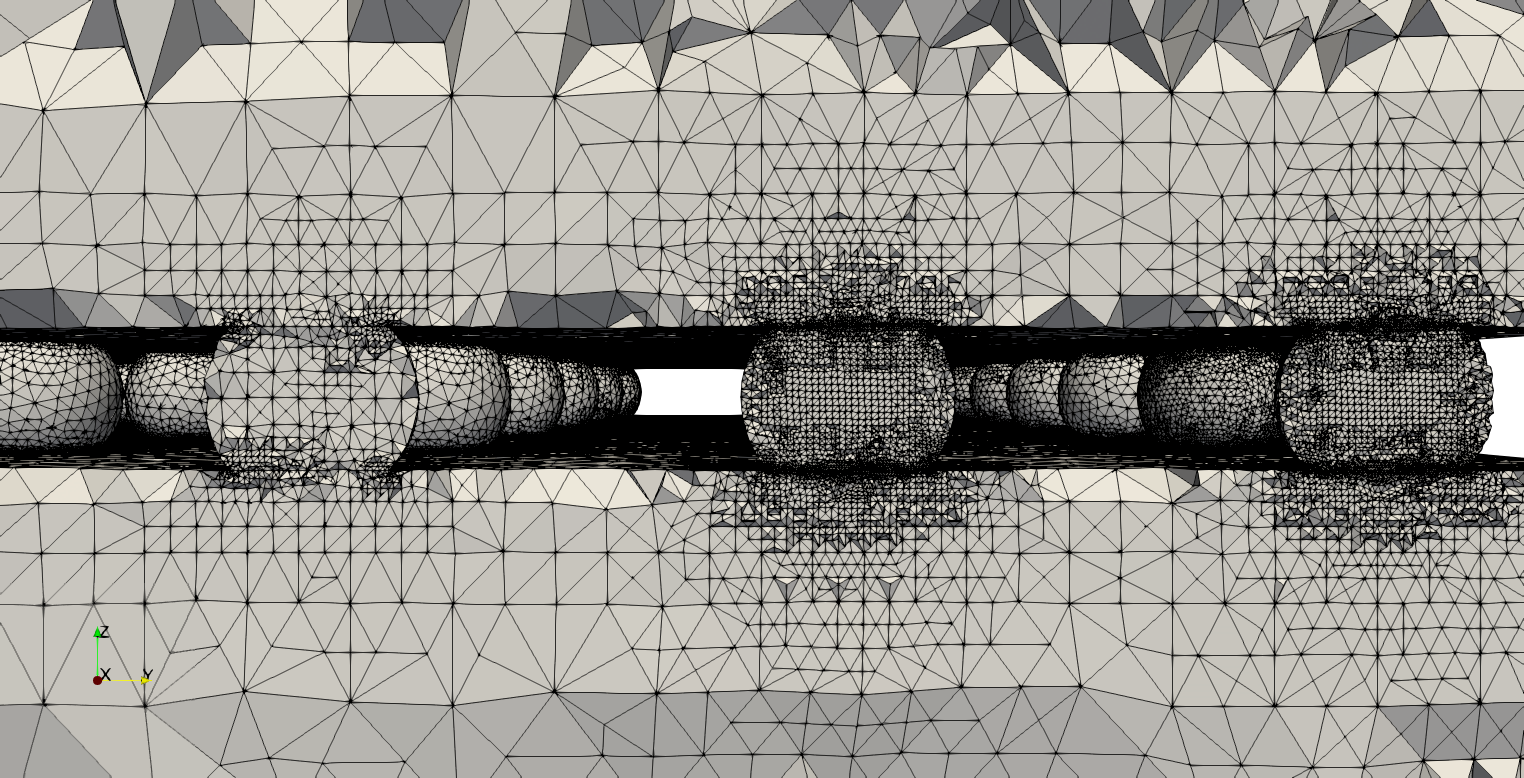
\includegraphics[width=.99\linewidth]{img/aut_solder_mesh_final.png}
\end{subfigure}%
\caption{Cross-sectional view of the initial mesh for the solder joint
geometry (left) and the final adapted mesh (right).}
\label{fig:aut_solder_mesh}
\end{figure}

\begin{figure}[ht!]
\centering
\begin{subfigure}{.5\textwidth}
\centering
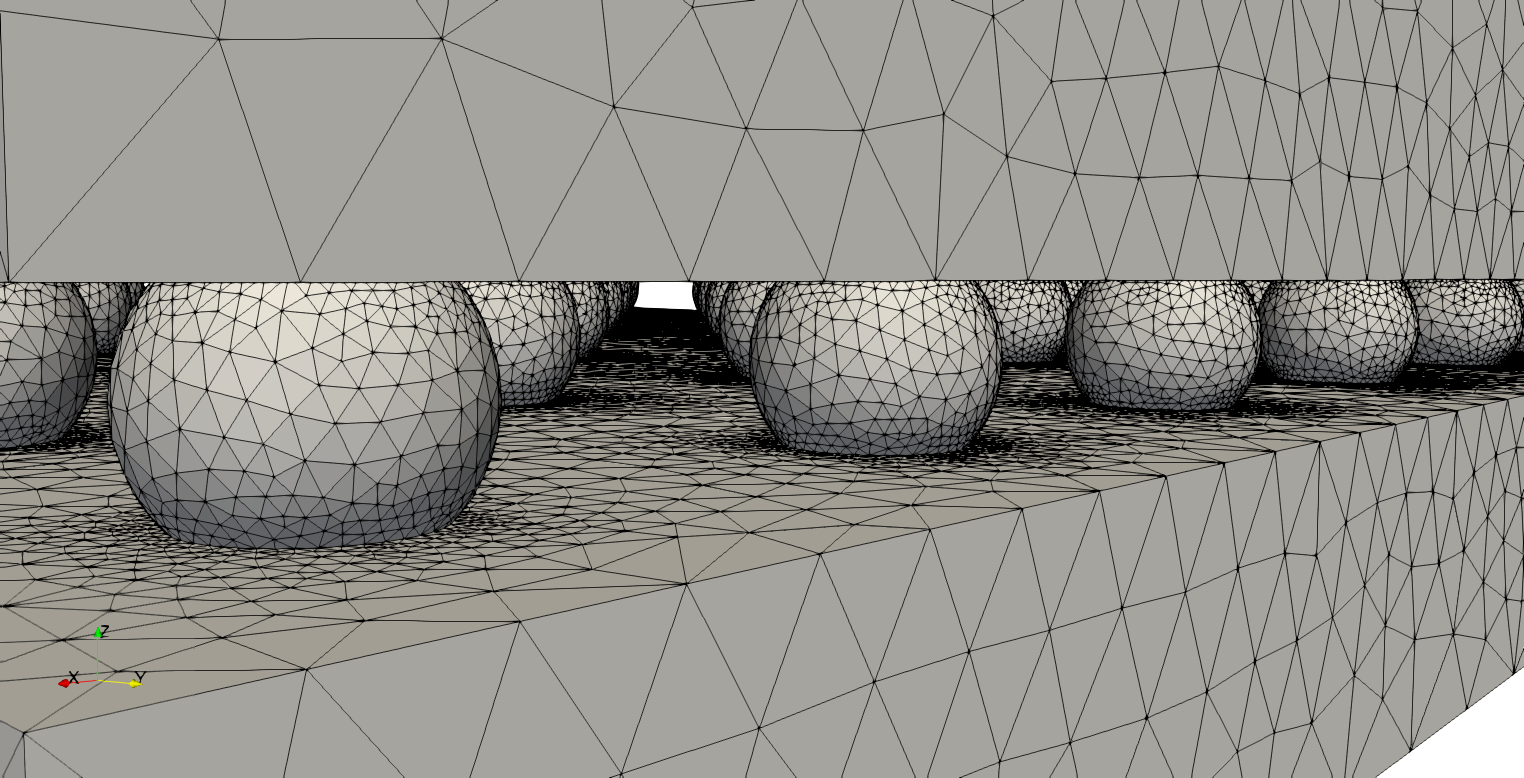
\includegraphics[width=.99\linewidth]{img/aut_solder_mesh_initial2.png}
\end{subfigure}%
\begin{subfigure}{0.5\textwidth}
\centering
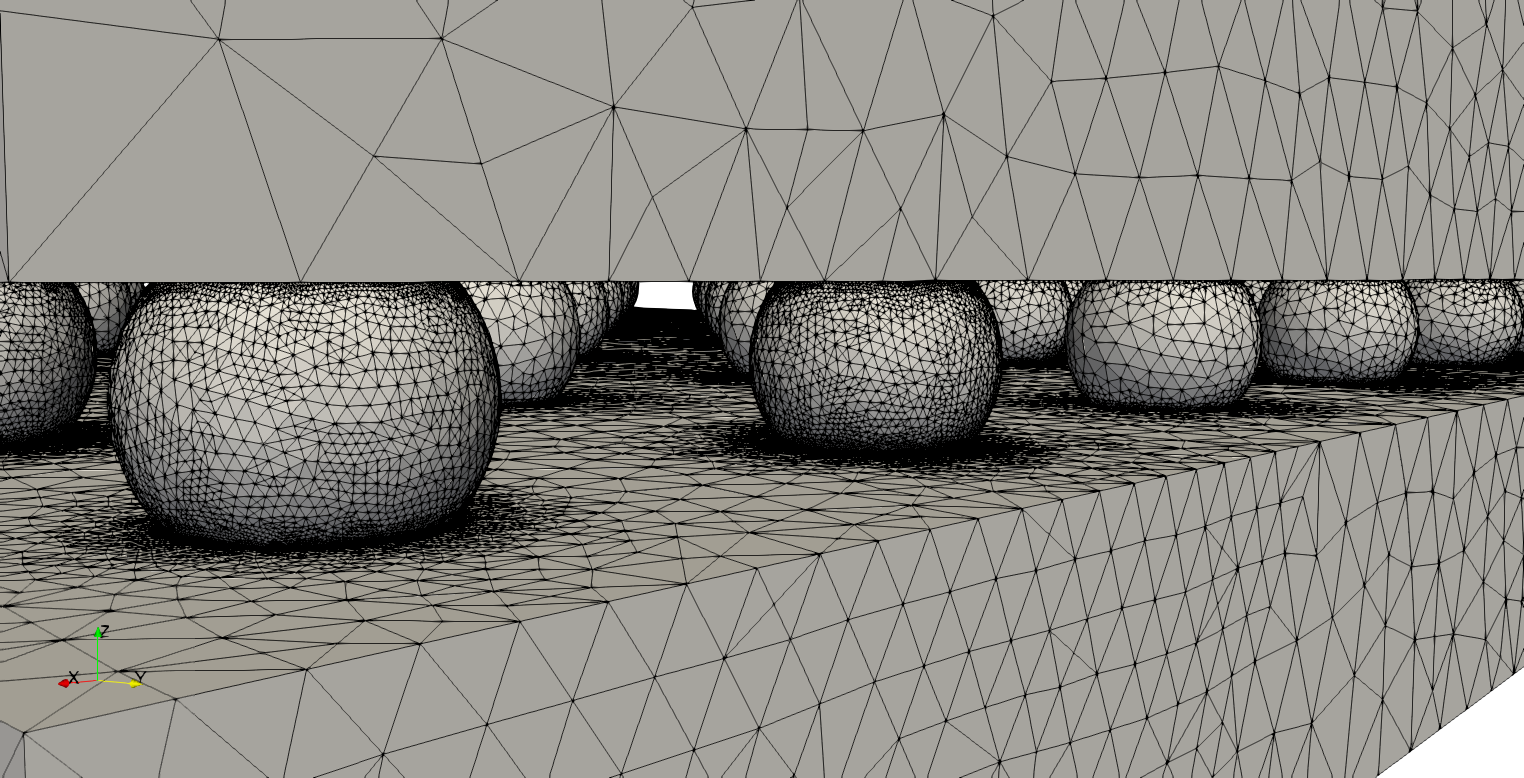
\includegraphics[width=.99\linewidth]{img/aut_solder_mesh_final2.png}
\end{subfigure}%
\caption{The initial mesh for the solder joint geometry (left) and the
final adapted mesh (right).}
\label{fig:aut_solder_mesh2}
\end{figure}

Figure \ref{fig:aut_solder_convergence} demonstrates the
convergence history of the error in the functional QoI,
as defined by the difference of the QoI obtained via
Richardson extrapolation and the QoI approximated by the
finite element solution. We compare the convergence for
two adaptive schemes, one achieved by successive uniform
refinements of the mesh and the other achieved by adjoint-based
error estimation. After 4 adaptive iterations, the adjoint-based
adaptive procedure achieves nearly the same degree of accuracy
as the uniform refinement procedure with two orders of
magnitude fewer degrees of freedom.

\begin{figure}[ht!]
\centering
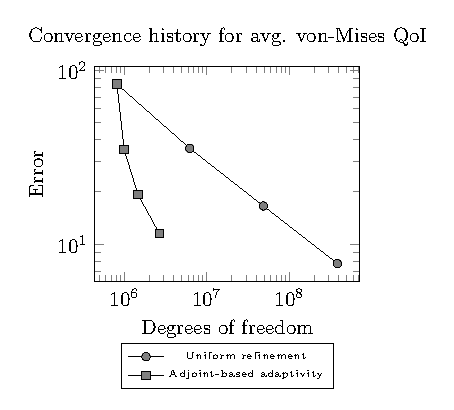
\includegraphics[width=0.5\linewidth]{img/aut_solder_convergence.pdf}
\caption{Error convergence histories for the solder joint example problem
with the average von-Mises stress QoI.}
\label{fig:aut_solder_convergence}
\end{figure}

Finally, we remark that automated parallel adaptive workflows
have been developed in reference \cite{bloomfield2017component}.
As an avenue for future investigation, adjoint-based error estimation
could be folded into these automated workflows.
In particular, an automated primal analysis could be used to inform
the actual selection of the QoI itself, which could then be accurately
assessed using adjoint-based error estimation.

%%% CONCLUSIONS
\section{Conclusions}

In this work, we have developed an automated approach for
adjoint-based error estimation and mesh adaptation for
execution on parallel machines. We have developed this approach
to be applicable to both Galerkin and stabilized finite
element methods. To realize this approach, we have extended
the concept of \emph{template-based generic programming} for
PDE models to include the automatic localization of error
contributions using a partition of unity-based
localization approach. We have demonstrated that this approach
is effective for a variety of example applications, including
nonlinear elasticity and elastoplasticity.
